\subsection{IFIT1, IFIT3, and IFIT5 Localisation with Regards to RSV Pseudo-IBs} \label{subsec:IFIT1, IFIT3, and IFIT5 Localisation with Regards to RSV Pseudo-IBs}


!!! To investigate the intreaction of IFITs with RSV pseudo inclusion bodies ... !!!

The cells, irrespective of the chosen cell line, were maintained and passaged under standard conditions, as outlined in Sections \ref{sec:Cell Culture} and \ref{subsec:Passaging and Seeding Cells}. Transfections involved the use of human or bovine RSV \textit{N} or \textit{P} codon-optimized ORFs, housed within pcDNA3.1 plasmid backbones, employing TransIT-X2 at a 1:2 ratio, as detailed in Section \ref{subsec:Transfecting Cells}. Despite attempts with lipofectamine 3000, which, although similar in transfection efficiencies, exhibited increased cellular toxicity (data not presented), we consistently utilized TransIT-X2 for transfection. The optimized conditions included transfecting 500 $\mu$g of each plasmid per 50,000 cells seeded in a 24-well plate per well, following experimentation and optimization of various parameters such as total DNA used, seeding density, and plasmid ratios (data not presented).

Initial experiments were conducted in human embryonic kidney (HEK) 293T cells, characterized by high plasmid transfection permissivity, often achieving efficiencies exceeding 90\%. However, these cells presented challenges for confocal microscopy and subsequent image analysis due to their small nucleus-to-cytoplasm ratio and adherence difficulties during treatment or washes. Despite these challenges, the initial IFIT1, and IFIT2 staining experiments (Section \ref{subsec:Dissecting the Differential IFIT2 Antibody Staining}) were conducted using HEK293T cells. Subsequently, a transition to alternative cell lines was deemed necessary. HeLa and Vero cell lines were evaluated based on their transfection efficiency, cell morphology, and culture simplicity. HeLa, derived from human uterine epithelial cancer cells, was considered more suitable for our purposes. In contrast, the Vero cell line originates from the kidney epithelial tissue of adult African green monkeys (\textit{Cercopithecus aethiops}) \cite{Simizu1967CharacterizationVero}. Initial optimization experiments revealed minimal transfection efficiency in the HeLa cell line under all tested conditions (data not shown). On the other hand, Vero cells consistently exhibited transfection, albeit with lower efficiencies compared to those observed in the HEK293T cell line (approximately 30\%/90\%, data not shown). Nevertheless, this level of transfection was deemed sufficient for subsequent confocal microscopy experiments.

Vero cells are commonly employed for propagating and studying various viruses, particularly bovine RSV. While the optimal scenario would involve detecting endogenous human IFITs interacting with RSV pseudo-inclusion bodies, it is crucial to note that primate IFITs, including those of monkeys, are phylogenetically more akin to human IFITs than bovine IFITs \cite{Zhou2013InterferonDefense}. As demonstrated in the previous chapter, the interactions of human and bovine IFITs exhibit considerable consistency. Therefore, exploring the colocalization of monkey IFITs with human or bovine pIBs holds promise for gaining valuable insights into these interactions.

\begin{figure}
    \begin{subfigure}{0.495\textwidth}
        \caption{}
        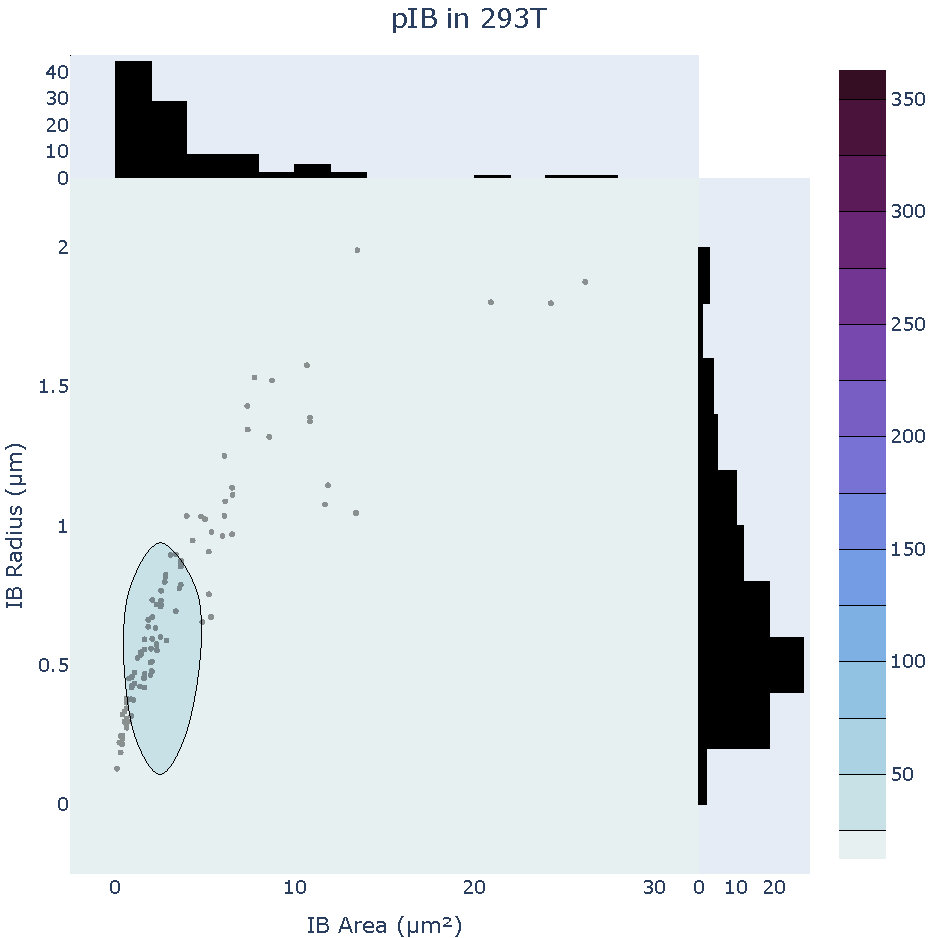
\includegraphics[width=\textwidth]{09. Chapter 4/Figs/01. pIB/01. pIB characterisation/01. heatmap_pib-293t.pdf} 
    \end{subfigure}
    \hfill
    \begin{subfigure}{0.495\textwidth}
        \caption{}
        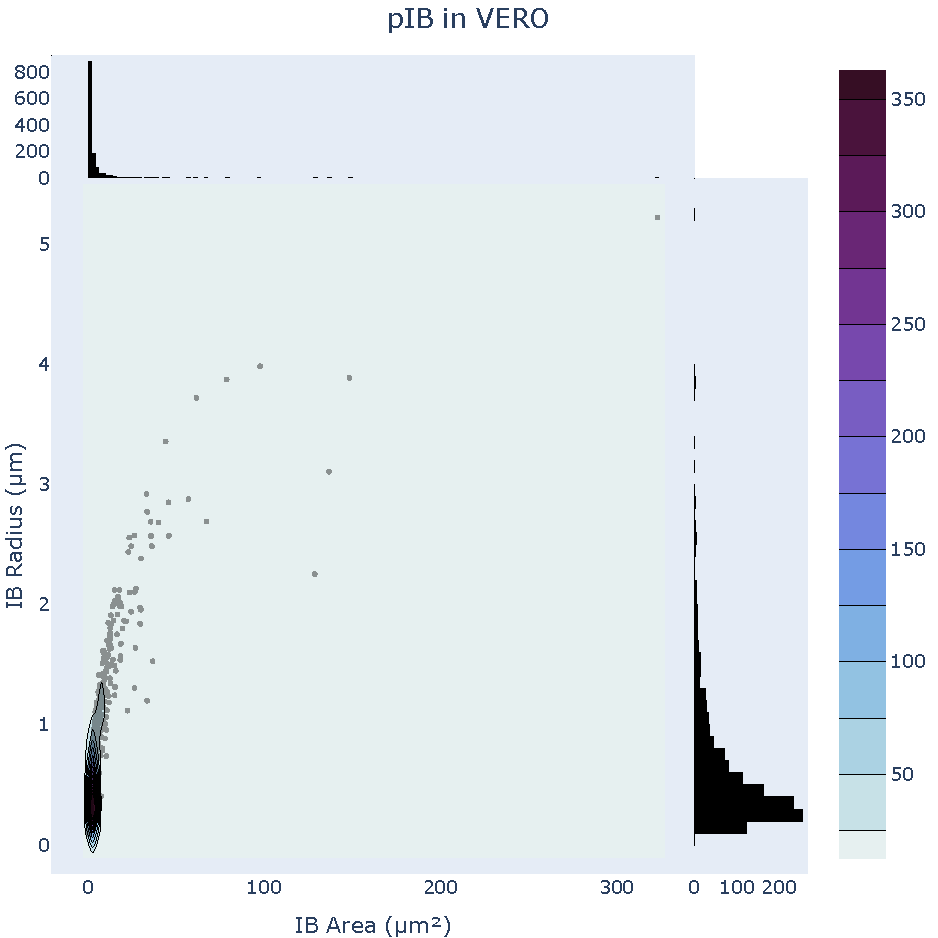
\includegraphics[width=\textwidth]{09. Chapter 4/Figs/01. pIB/01. pIB characterisation/02. heatmap_pib-vero.pdf}
    \end{subfigure}
    \caption[Size Characterisation of Pseudo Inclusion Bodies Across Different Cell Lines.]{\textbf{Size Characterisation of Pseudo Inclusion Bodies Across Different Cell Lines.} This figure presents the relationship between the measured area (\(\mu \mbox{m}^2\)) and diameter (\(\mu \mbox{m}\)) of individual pseudo inclusion bodies (pIBs) as observed within the scope of this study. Additionally, the figure includes distinct population distributions depicted alongside the plots, representing (a) 103 observations from the 293T cell line and (b) 1321 observations from the Vero cell line. Contour plots are incorporated to elucidate the underlying density of individual IBs within the plots.}
    \label{fig:Size Characterisation of Pseudo Inclusion Bodies Across Different Cell Lines}
\end{figure}

We conducted a systematic observation and annotation of a total of 1424 pseudo-inclusion bodies, comprising 103 observations in the HEK293T cell line and 1321 observations in the Vero cell line. The relationship between their measured area and radius is illustrated in Figure \ref{fig:Size Characterization of Pseudo-Inclusion Bodies Across Different Cell Lines}. Pseudo-inclusion bodies in both cell lines generally conform to logarithmic curves, consistent with the expected relationship of the observed values. Notably, a substantial number of detected entities exhibit a larger measured area than the predicted radius, indicative of an elongated ellipsoidal shape. In the HEK293T cell line, the pseudo-inclusion bodies predominantly displayed a radius of 0.5 \(\mu \mbox{m}\), with the majority falling within the range of 0.25 \(\mu \mbox{m}\) to 1 \(\mu \mbox{m}\). Regarding the associated measured area, most pseudo-inclusion bodies ranged from 0.5 \(\mu \mbox{m}^2\) to 4 \(\mu \mbox{m}^2\). Contrastingly, in the Vero cell line, we observed a broader distribution of data, with pseudo-inclusion bodies measuring >5 \(\mu \mbox{m}\) in radius and >300 \(\mu \mbox{m}^2\) in area. Nevertheless, the majority of the detected entities in this cell line exhibited radii between 0.1 \(\mu \mbox{m}\) and 0.7 \(\mu \mbox{m}\), coupled with measured 2D areas ranging from 0.1 \(\mu \mbox{m}^2\) to 4 \(\mu \mbox{m}^2\).

\begin{figure}
    \centering
    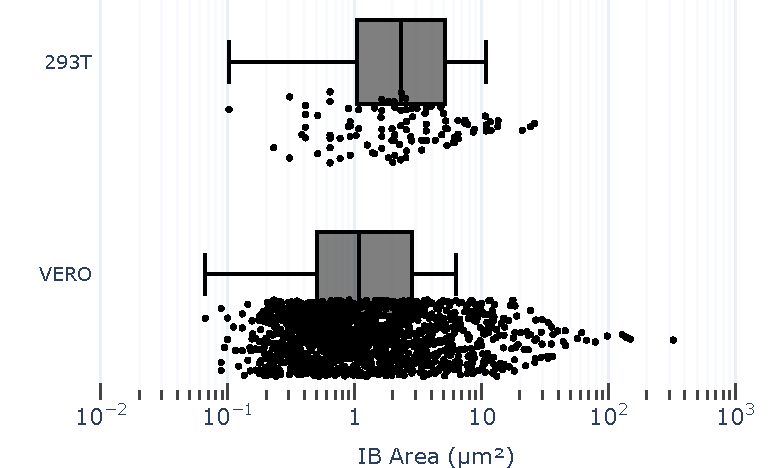
\includegraphics[width=0.75\linewidth]{09. Chapter 4/Figs/01. pIB/01. pIB characterisation/03. box-pib.pdf}
    \caption[The Distributions of pIB Areas Observed Per Cell Line.]{\textbf{The Distributions of pIB Areas Observed Per Cell Line.} The distribution of RSV pseudo inclusion body areas (\(\mu \mbox{m}^2\)), detected in this study are shown. A total of 103 observations were made in the 293T cell line, and 1321 observations in the Vero cell line.}
    \label{fig:The Distributions of pIB Areas Observed Per Cell Line}
\end{figure}

A more detailed view focusing solely on the distribution of measured areas per cell line can be observed in Figure \ref{fig:The Distributions of pIB Areas Observed Per Cell Line}. Notably, pIBs detected in the Vero cell line exhibit a broader range in terms of minimal and maximal measured areas compared to those in the 293T cell line. However, the median value in the 293T cell line surpasses that of the Vero cell line. Specifically, in the 293T cell line, we observed pIB areas ranging from sub 0.2 \(\mu \mbox{m}^2\) to supra 20 \(\mu \mbox{m}^2\), with a median value of 2.2 \(\mu \mbox{m}^2\). Conversely, in the Vero cell line, the observed pIBs spanned from sub 0.07 \(\mu \mbox{m}^2\) to supra 300 \(\mu \mbox{m}^2\), with a median value of 1 \(\mu \mbox{m}^2\). It is noteworthy that both median values are notably smaller than those observed in cell lines during infection (refer to Section \ref{subsec:IFIT Subcellular Localization During Interferon Induction and RSV Infection}, Figure \ref{fig:The Distributions of IB Areas Observed Per Cell Line}). This finding aligns with literature reports, indicating that pIBs observed 24 hours post-transfection are considerably smaller than conventional inclusion bodies observed in infected cells after an equivalent passage of time \cite{Jobe2021BovineResponses}.

\begin{figure}
    \begin{subfigure}{0.495\textwidth}
        \caption{}
        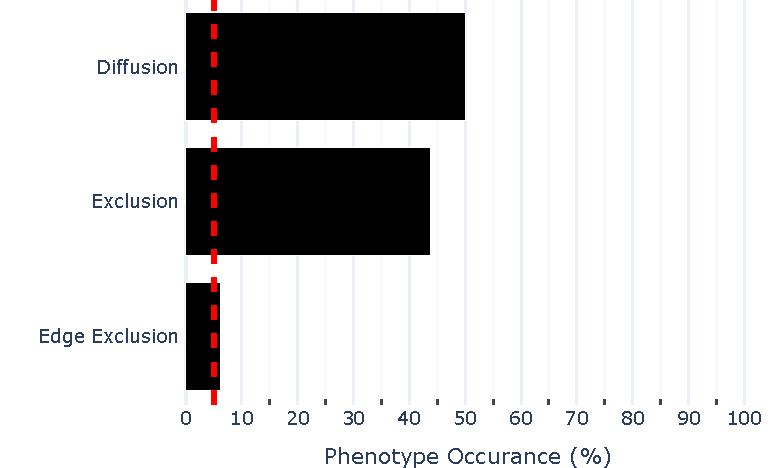
\includegraphics[width=1\linewidth]{09. Chapter 4/Figs/01. pIB/02. IFIT1/01. bar_i1_293t.pdf} 
    \end{subfigure}
    \begin{subfigure}{0.495\textwidth}
        \caption{}
        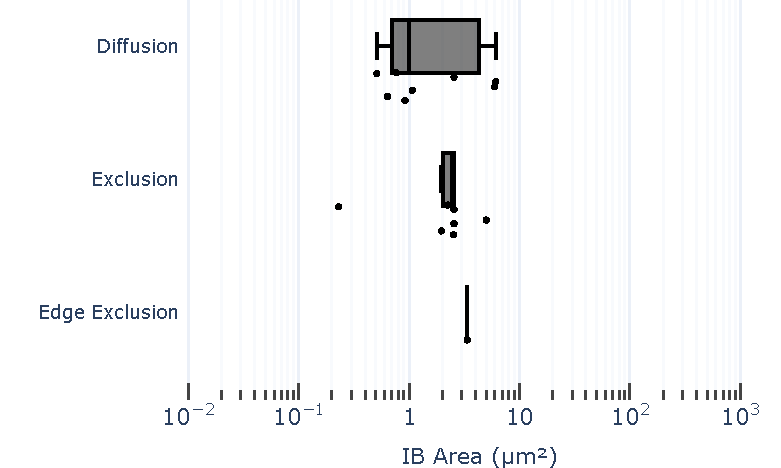
\includegraphics[width=1\linewidth]{09. Chapter 4/Figs/01. pIB/02. IFIT1/02. box_i1_293t.pdf}
    \end{subfigure}
    \caption[Phenotypic Interactions of Human IFIT1 with Human pIBs in the 293T Cell Line.]{\textbf{Phenotypic Interactions of Human IFIT1 with Human pIBs in the 293T Cell Line.} 293T cells were transfected with hRSV N and P containing plasmids using TransIT-X2 and were fixed after 24 hours. Cells were labeled with anti-RSV N and anti-IFIT1 antibodies and imaged on confocal microscope. Panel (a) shows percentual proportions of observed phenotypes between hRSV pseudo inclusion bodies and human IFIT1 (16 observations), with the red dotted line denoting the 5\% threshold, marking phenotypes considered relevant above this limit. Panel (b) shows the IB area in \(\mu \mbox{m}^2\) per observed relevant phenotype.}
    \label{fig:Phenotypic Interactions of Human IFIT1 with Human pIBs in the 293T Cell Line}
\end{figure}

\begin{figure}
    \centering
    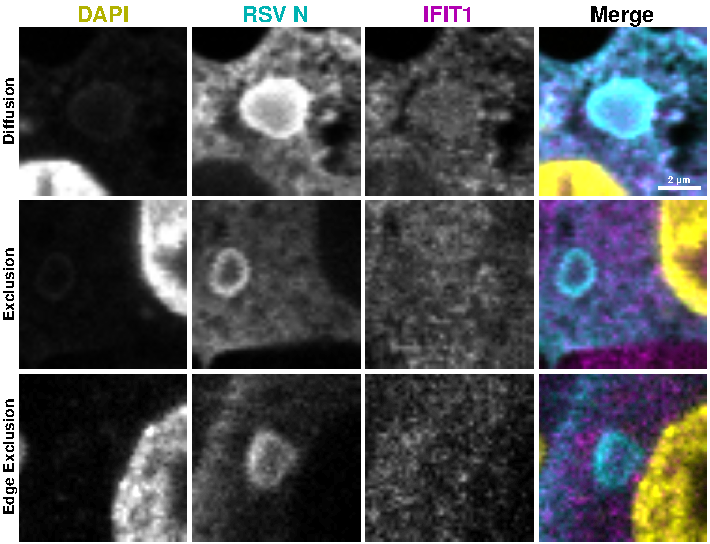
\includegraphics[width=1\linewidth]{09. Chapter 4/Figs/01. pIB/02. IFIT1/03. i1-293t-hnhp.pdf}
    \caption[Representative Images of Phenotypic Interactions of Human IFIT1 with Human pIBs in the 293T Cell Line.]{\textbf{Representative Images of Phenotypic Interactions of Human IFIT1 with Human pIBs in the 293T Cell Line.} 293T cells were transfected with hRSV N and P containing plasmids using TransIT-X2 and were fixed after 24 hours. Cellular nuclei were stained with DAPI (yellow), and cells were double-labeled with anti-RSV N (cyan) and anti-IFIT1 (magenta) antibodies. This figure showcases representative examples of relevant phenotypes in the interaction between human IFIT1 and hRSV pseudo inclusion bodies. These phenotypes are presented in descending order based on their percentage proportions. The scale bar indicates 2 \(\mu \mbox{m}\).}
    \label{fig:Representative Images of Phenotypic Interactions of Human IFIT1 with Human pIBs in the 293T Cell Line}
\end{figure}

We obtained 16 observations of endogenous human IFIT1 and its interaction with hRSV pIBs in the 293T cell line. The observed phenotype frequencies, along with the measured pIB sizes, can be viewed in Figure \ref{fig:Phenotypic Interactions of Human IFIT1 with Human pIBs in the 293T Cell Line}, with representative images of these phenotypes shown in Figure \ref{fig:Representative Images of Phenotypic Interactions of Human IFIT1 with Human pIBs in the 293T Cell Line}. Half of the observations displayed the diffusion phenotype. This was predominantly observed in smaller pIBs with a typical size of 1 \(\mu \mbox{m}^2\) and ranging from 0.5 \(\mu \mbox{m}^2\) to 6 \(\mu \mbox{m}^2\) in size. The second most prevalent phenotype was exclusion, which occurred in 44\% of cases. The pIBs associated with this phenotype closely clustered at around 2.5 \(\mu \mbox{m}^2\), with two exceptions, i.e., one very small pIB (0.22 \(\mu \mbox{m}^2\)) and one relatively large pIB (5 \(\mu \mbox{m}^2\)). Lastly, we observed one pIB with a measured area of 3.3 \(\mu \mbox{m}^2\) which exhibited the exclusion phenotype. Overall, these data suggest that human IFIT1 does not associate with human RSV pIB structures, although this is based on a very limited set of observations.

\begin{figure}
    \begin{subfigure}{0.495\textwidth}
        \caption{}
        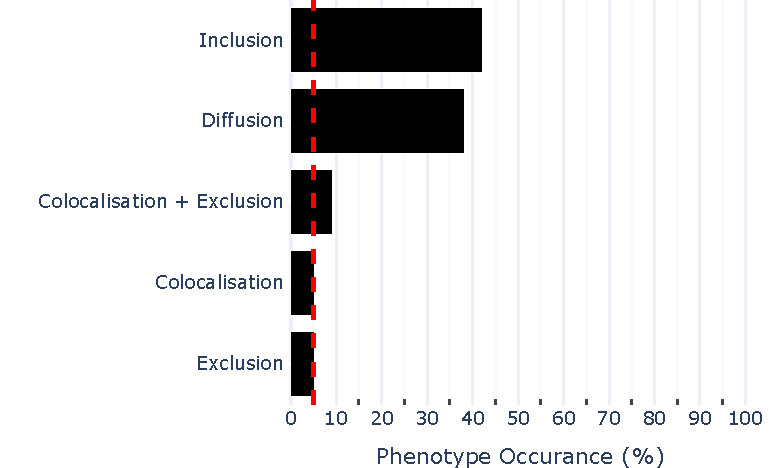
\includegraphics[width=1\linewidth]{09. Chapter 4/Figs/01. pIB/02. IFIT1/04. bar_i1_vero_hnhp.pdf} 
    \end{subfigure}
    \begin{subfigure}{0.495\textwidth}
        \caption{}
        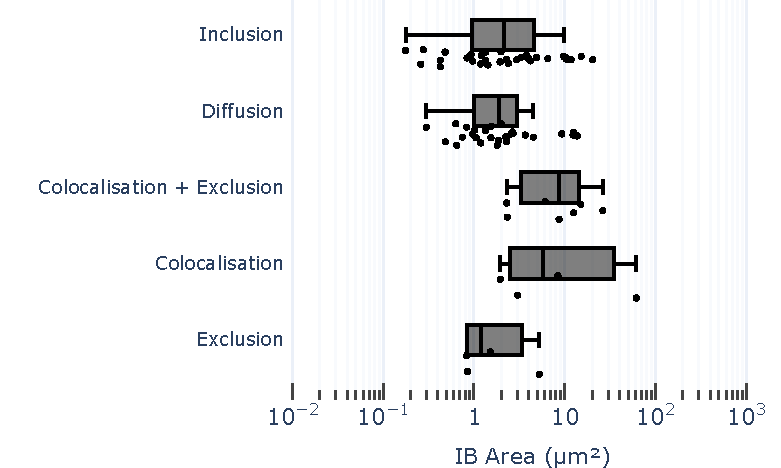
\includegraphics[width=1\linewidth]{09. Chapter 4/Figs/01. pIB/02. IFIT1/05. box_i1_vero_hnhp.pdf}
    \end{subfigure}
    \caption[Interaction Phenotypes of Monkey IFIT1 with Human pIBs in the Vero Cell Line.]{\textbf{Interaction Phenotypes of Monkey IFIT1 with Human pIBs in the Vero Cell Line.} Vero cells were transfected with hRSV N and P containing plasmids using TransIT-X2 and were fixed after 24 hours. Cells were labeled with anti-RSV N and anti-IFIT1 antibodies and imaged on confocal microscope. Panel (a) shows percentual proportions of observed phenotypes between hRSV pseudo inclusion bodies and monkey IFIT1 (76 observations), with the red dotted line denoting the 5\% threshold, marking phenotypes considered relevant above this limit. Panel (b) shows the IB area in \(\mu \mbox{m}^2\) per observed relevant phenotype.}
    \label{fig:Interaction Phenotypes of Monkey IFIT1 with Human pIBs in the VERO Cell Line}
\end{figure}

\begin{figure}
    \centering
    \includegraphics[width=1\linewidth]{09. Chapter 4/Figs/01. pIB/02. IFIT1/06. i1-vero-hnhp.pdf}
    \caption[Representative Images of Interaction Phenotypes of Monkey IFIT1 with Human pIBs in the Vero Cell Line.]{\textbf{Representative Images of Interaction Phenotypes of Monkey IFIT1 with Human pIBs in the Vero Cell Line.} Vero cells were transfected with hRSV N and P containing plasmids using TransIT-X2 and were fixed after 24 hours. Cellular nuclei were stained with DAPI (yellow), and cells were double-labeled with anti-RSV N (cyan) and anti-IFIT1 (magenta) antibodies. This figure showcases representative examples of relevant phenotypes in the interaction between monkey IFIT1 and hRSV pseudo inclusion bodies. These phenotypes are presented in descending order based on their percentage proportions. The scale bar indicates 2 \(\mu \mbox{m}\).}
    \label{fig:Representative Images of Interaction Phenotypes of Monkey IFIT1 with Human pIBs in the VERO Cell Line}
\end{figure}

Next, we evaluated endogenous monkey IFIT1 interactions with pIBs created by transfection of hRSV \textit{N} and \textit{P} containing plasmids in the Vero cell line. The frequencies of occurrences of the interaction phenotypes based on 76 observations, along with the measured pIB areas per phenotype, are shown in Figure \ref{fig:Interaction Phenotypes of Monkey IFIT1 with Human pIBs in the VERO Cell Line}. Representative images of these phenotypes are shown in Figure \ref{fig:Representative Images of Interaction Phenotypes of Monkey IFIT1 with Human pIBs in the VERO Cell Line}. A notable 43\% of the observations depicted monkey IFIT1 forming intra-pIB inclusion, followed closely by a diffusion phenotype, observed in 38\% of instances. Further, 8\% of the observations revealed monkey IFIT1 colocalizing with the edge of the pIB structure while being excluded from the primary pIB structure. Both colocalization and exclusion phenotypes individually occurred in 5\% of cases each. Regarding the size profile of hRSV pIBs associated with these phenotypes, inclusion was observed across a diverse range of pIB sizes, spanning from sub 0.2 \(\mu \mbox{m}^2\) to supra 20 \(\mu \mbox{m}^2\), with a median size of 2 \(\mu \mbox{m}^2\). In contrast, the diffusion phenotype occured in pIBs with a similar range of measured areas, displaying an identical median value of 2 \(\mu \mbox{m}^2\). Noteworthy distinctions emerged in the distribution of values between these two phenotypes. While the sizes of pIBs associated with the inclusion phenotype were evenly distributed across their minimal and maximal values, those linked with the diffusion phenotype clustered around 2 \(\mu \mbox{m}^2\). The colocalisation associated with the pIB exclusion phenotype occurred predominantly in larger pIBs, with a typical area of 9 \(\mu \mbox{m}^2\), absent in pIBs smaller than 2 \(\mu \mbox{m}^2\). Similarly, the colocalisation-phenotype associated hRSV pIBs exhibited larger sizes, with a median value of 6 \(\mu \mbox{m}^2\) and a minimal value of 2 \(\mu \mbox{m}^2\). Lastly, the exclusion phenotype occured in 4 pIBs with a median 2D area of 1.1 \(\mu \mbox{m}^2\). In summary, within this simplified model, although the size of the pIB should not directly indicate a difference in the underlying pIB complexity, we observed a size-dependent association with phenotypes. Smaller, sub 1 \(\mu \mbox{m}^2\) pIBs predominantly exhibited inclusion and diffusion phenotypes, equally prevalent in these structures. In contrast, larger pIBs showcased inclusion, diffusion, and colocalisation associated with exclusion.

\begin{figure}
    \begin{subfigure}{0.495\textwidth}
        \caption{}
        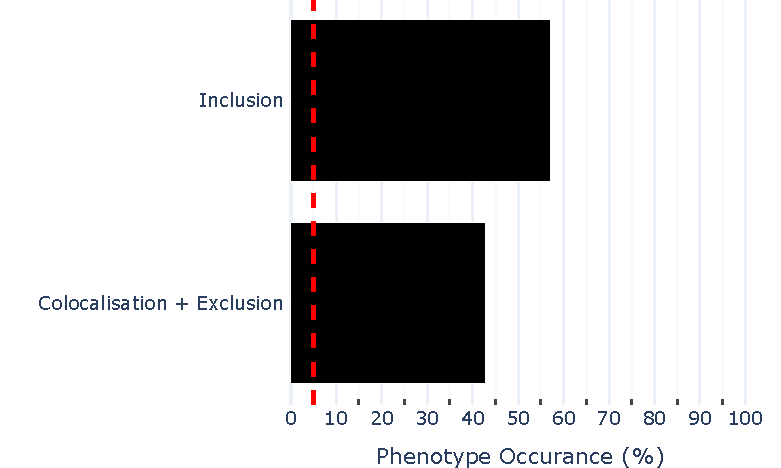
\includegraphics[width=1\linewidth]{09. Chapter 4/Figs/01. pIB/02. IFIT1/07. bar_i1_vero_bnbp.pdf}  
    \end{subfigure}
    \begin{subfigure}{0.495\textwidth}
        \caption{}
        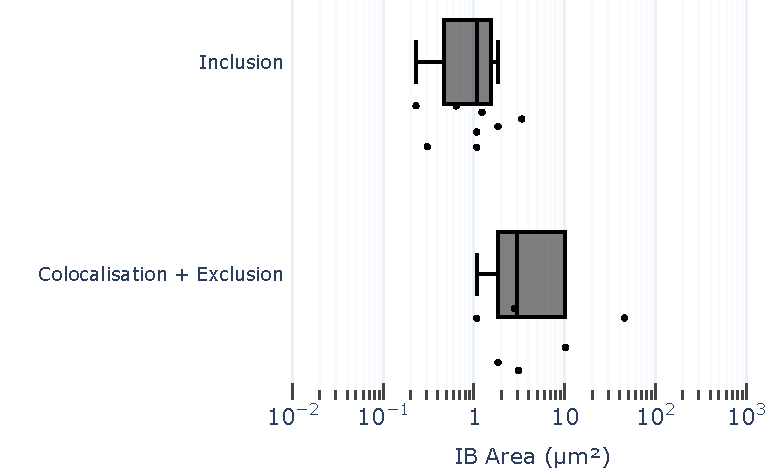
\includegraphics[width=1\linewidth]{09. Chapter 4/Figs/01. pIB/02. IFIT1/08. box_i1_vero_bnbp.pdf}
    \end{subfigure}
    \caption[Interaction Phenotypes of Monkey IFIT1 with Bovine pIBs in the Vero Cell Line.]{\textbf{Interaction Phenotypes of Monkey IFIT1 with Bovine pIBs in the Vero Cell Line.} Vero cells were transfected with bRSV N and P containing plasmids using TransIT-X2 and were fixed after 24 hours. Cells were labeled with anti-RSV N and anti-IFIT1 antibodies and imaged on confocal microscope. Panel (a) shows percentual proportions of observed phenotypes between bRSV pseudo inclusion bodies and monkey IFIT1 (14 observations), with the red dotted line denoting the 5\% threshold, marking phenotypes considered relevant above this limit. Panel (b) shows the IB area in \(\mu \mbox{m}^2\) per observed relevant phenotype.}
    \label{fig:Interaction Phenotypes of Monkey IFIT1 with Bovine pIBs in the VERO Cell Line}
\end{figure}

\begin{figure}
    \centering
    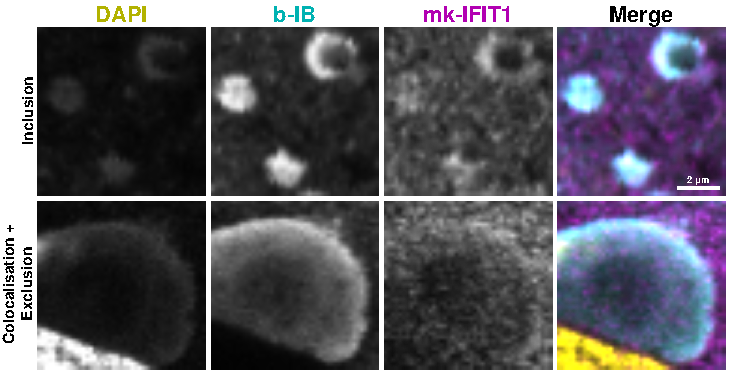
\includegraphics[width=1\linewidth]{09. Chapter 4/Figs/01. pIB/02. IFIT1/09. i1-vero-bnbp.pdf}
    \caption[Representative Images of Interaction Phenotypes of Monkey IFIT1 with Bovine pIBs in the Vero Cell Line.]{\textbf{Representative Images of Interaction Phenotypes of Monkey IFIT1 with Bovine pIBs in the Vero Cell Line.} Vero cells were transfected with bRSV N and P containing plasmids using TransIT-X2 and were fixed after 24 hours. Cellular nuclei were stained with DAPI (yellow), and cells were double-labeled with anti-RSV N (cyan) and anti-IFIT1 (magenta) antibodies. This figure showcases representative examples of relevant phenotypes in the interaction between monkey IFIT1 and bRSV pseudo inclusion bodies. These phenotypes are presented in descending order based on their percentage proportions. The scale bar indicates 2 \(\mu \mbox{m}\).}
    \label{fig:Representative Images of Interaction Phenotypes of Monkey IFIT1 with Bovine pIBs in the VERO Cell Line}
\end{figure}

In the final exploration, we examined the interaction of monkey IFIT1, detected by the human IFIT1 antibody, with bovine RSV IBs through the transfection of bRSV \textit{N} and \textit{P} containing plasmids. Challenges arose due to consistently lower transfection efficiencies associated with these plasmids, resulting in a limited number of observations. Consequently, we encountered difficulties in generating sufficient samples to investigate endogenous monkey IFITs other than IFIT1 and IFIT2 using the A antibody, as detailed in Section \ref{subsec:Dissecting the Differential IFIT2 Antibody Staining}. Nonetheless, Figure \ref{fig:Interaction Phenotypes of Monkey IFIT1 with Bovine pIBs in the VERO Cell Line} presents the frequencies of occurrence of interaction phenotypes based on 14 observations, coupled with the measured pIB areas per phenotype. Representative images of these phenotypes are displayed in Figure \ref{fig:Representative Images of Interaction Phenotypes of Monkey IFIT1 with Bovine pIBs in the VERO Cell Line}. Remarkably, a pattern reminiscent of IFIT2 during RSV infection emerged, where only two phenotypes were observed: inclusion within the pIB structures, occurring at a frequency of 56\%, and colocalisation associated with pIB exclusion, occurring at a frequency of 44\%. The former predominated in smaller pIBs, with a median size of 1 \(\mu \mbox{m}^2\) and a maximum size of 4 \(\mu \mbox{m}^2\). In contrast, the colocalisation phenotype associated with exclusion manifested in pIBs with a typical size of 3 \(\mu \mbox{m}^2\). Despite an overlap in pIB sizes between the two phenotypes, sub 1 \(\mu \mbox{m}^2\) pIBs consistently correlated with inclusion, while supra 10 \(\mu \mbox{m}^2\) pIBs were consistently associated with colocalisation conjoined with exclusion.

Considering the entirety of the IFIT1-pIB interaction results, it suggests a differential propensity for pIB interaction between endogenous human and monkey IFIT1. NSaying that, data obtained from the HEK293T cell line is limited in quantity and displays a size bias towards pIBs that are less than 6 \(\mu \mbox{m}^2\) in size. This observation does not align with the true diversity of pIB sizes observed in this study, as the aggregate of all pIBs observed in HEK293T cells indicates a sizable population of supra 6 \(\mu \mbox{m}^2\) pIBs (Figure \ref{fig:The Distributions of pIB Areas Observed Per Cell Line}). In the Vero cell line transfected with hRSV \textit{N} and \textit{P} ORF-containing plasmids, we have observed phenotypes that imply direct interaction (colocalisation and colocalisation associated with exclusion) specifically in larger pIBs. This implies that the limited sample size and diversity of HEK293T observed hRSV pIBs are not sufficient to provide a true picture of IFIT1/pIB interaction. On the other hand, it can also be indicative of hIFIT1 not being recruited to the pIBs. Within the Vero cell line, we also observed differential results which depend on the species of the virus. While we have only observed direct interaction phenotypes of inclusion formation and pIB edge colocalisation with intra-pIB exclusion with the bRSV pIBs, we observed a more diverse interaction range in Vero cells with hRSV pIBs present in them. These phenotypes, however, all, with the exception of exclusion phenotype (which occurred only in 5\% of observations), imply IFIT1 having access to the pIB structure. It is intriguing to see the differences between human and bovine RSV pIB and their interaction with monkey IFIT1. This could suggest that the bovine pIB possibly lack a mechanism that would prevent them from being targeted by the monkey IFIT1. Saying that, the bovine RSV pIB dataset lacks in-depth with regards to the amount of observations, and thus the differences could also be attributed to the low frequency of diffusion or exclusion phenotypes. In that case, the results from Vero cell lines with either human or bovine RSV pIBs present would be almost identical.

\begin{figure}
    \begin{subfigure}{0.495\textwidth}
        \caption{}
        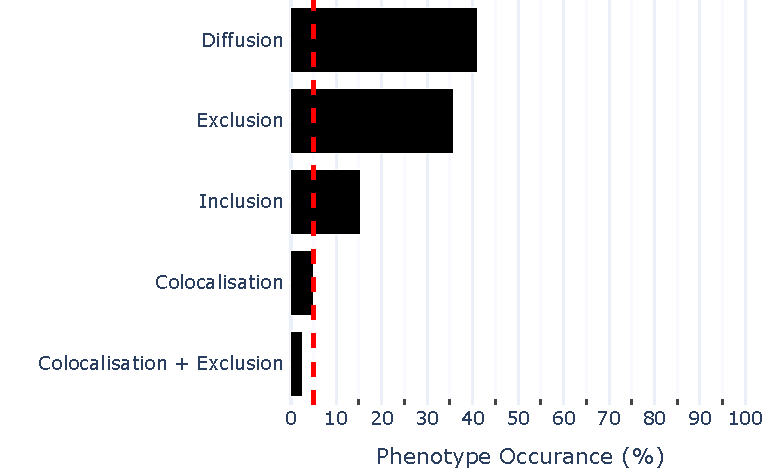
\includegraphics[width=1\linewidth]{09. Chapter 4/Figs/01. pIB/04. IFIT3/01. bar_i3_vero.pdf} 
    \end{subfigure}
    \begin{subfigure}{0.495\textwidth}
        \caption{}
        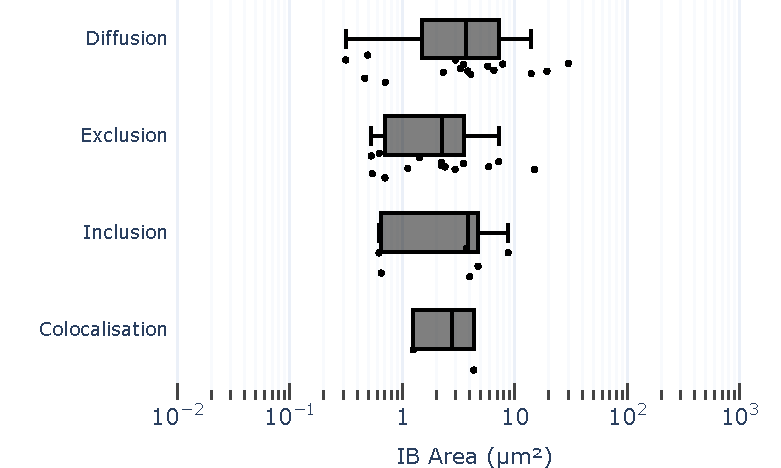
\includegraphics[width=1\linewidth]{09. Chapter 4/Figs/01. pIB/04. IFIT3/02. box_i3_vero.pdf}
    \end{subfigure}
    \caption[Interaction Phenotypes of Monkey IFIT3 with Human pIBs in the Vero Cell Line.]{\textbf{Interaction Phenotypes of Monkey IFIT3 with Human pIBs in the Vero Cell Line.} Vero cells were transfected with hRSV N and P containing plasmids using TransIT-X2 and were fixed after 24 hours. Cells were labeled with anti-RSV N and anti-IFIT3 antibodies and imaged on confocal microscope. Panel (a) shows percentual proportions of observed phenotypes between hRSV pseudo inclusion bodies and monkey IFIT3 (39 observations), with the red dotted line denoting the 5\% threshold, marking phenotypes considered relevant above this limit. Panel (b) shows the IB area in \(\mu \mbox{m}^2\) per observed relevant phenotype.}
    \label{fig:Interaction Phenotypes of Monkey IFIT3 with Human pIBs in the VERO Cell Line}
\end{figure}

\begin{figure}
    \centering
    \includegraphics[width=1\linewidth]{09. Chapter 4/Figs/01. pIB/04. IFIT3/03. i3-vero-hnhp.pdf}
    \caption[Representative Images of Interaction Phenotypes of Monkey IFIT3 with Human pIBs in the Vero Cell Line.]{\textbf{Representative Images of Interaction Phenotypes of Monkey IFIT3 with Human pIBs in the Vero Cell Line.} Vero cells were transfected with hRSV N and P containing plasmids using TransIT-X2 and were fixed after 24 hours. Cellular nuclei were stained with DAPI (yellow), and cells were double-labeled with anti-RSV N (cyan) and anti-IFIT3 (magenta) antibodies. This figure showcases representative examples of relevant phenotypes in the interaction between monkey IFIT3 and hRSV pseudo inclusion bodies. These phenotypes are presented in descending order based on their percentage proportions. The scale bar indicates 2 \(\mu \mbox{m}\).}
    \label{fig:Representative Images of Interaction Phenotypes of Monkey IFIT3 with Human pIBs in the VERO Cell Line}
\end{figure}

Next, we explored the interaction of IFIT3 with RSV pseudo-inclusion bodies. Unfortunately, attempts to generate samples comprising both HEK293T cells transfected with hRSV \textit{N} and \textit{P}, and Vero cells transfected with bRSV \textit{N} and \textit{P} for staining with IFIT3 were unsuccessful. Consequently, we present the analysis of monkey IFIT3 interaction with hRSV pIBs. The frequencies of observed phenotypes within 39 observations, along with the measured pIB sizes per phenotype occurring with more than 5\% frequency, are depicted in Figure \ref{fig:Interaction Phenotypes of Monkey IFIT3 with Human pIBs in the VERO Cell Line}. Representative images of phenotypes occurring with at least 5\% frequency are shown in Figure \ref{fig:Representative Images of Interaction Phenotypes of Monkey IFIT3 with Human pIBs in the VERO Cell Line}. The most prevalent phenotype is diffusion throughout the pIB structure, occurring in 41\% of observations. This is closely followed by an exclusion phenotype, observed in 36\% of cases. Monkey IFIT3 forming intra-pIB inclusions was observed in 15\% of cases. Lastly, 5\% of observations showed a colocalisation phenotype, while 3\% displayed colocalisation associated with exclusion. Regarding the size profile of the IBs associated with different phenotypes occurring with at least 5\% frequency, their median values seem quite similar. However, they encompass a progressively narrower range of values as the occurrence frequency decreases. In more detail, the diffusion phenotype median pIB size was 4 \(\mu \mbox{m}^2\), ranging from 0.3 \(\mu \mbox{m}^2\) to 30 \(\mu \mbox{m}^2\). The exclusion phenotype-associated median area value was 2 \(\mu \mbox{m}^2\), with detected pIB sizes ranging from sub-0.6 \(\mu \mbox{m}^2\) to supra-10 \(\mu \mbox{m}^2\). The size values of inclusion-associated pIBs clustered at around 3 \(\mu \mbox{m}^2\), ranging from two observations at 6 \(\mu \mbox{m}^2\) to one observation at 9 \(\mu \mbox{m}^2\). Lastly, the pIBs associated with the colocalisation phenotype had sizes of 1.3 \(\mu \mbox{m}^2\) and 4.3 \(\mu \mbox{m}^2\). In most cases, monkey IFIT3 does not appear to directly interact with hRSV pIB structures. However, in a quarter of the cases, it either forms inclusions or associates with the edge of the pIB structure. This data aligns with our earlier investigation where IFIT3 predominantly exhibited exclusion and diffusion phenotypes during RSV infection.

\begin{figure}
    \begin{subfigure}{0.495\textwidth}
        \caption{}
        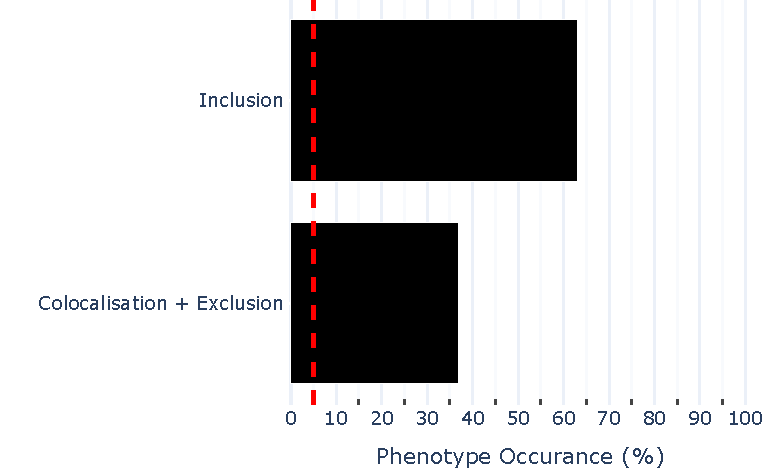
\includegraphics[width=1\linewidth]{09. Chapter 4/Figs/01. pIB/05. IFIT5/01. bar_i5_vero.pdf} 
    \end{subfigure}
    \begin{subfigure}{0.495\textwidth}
        \caption{}
        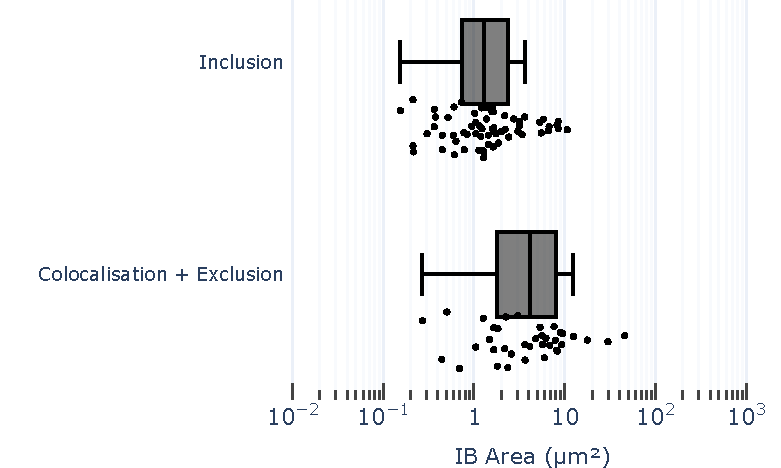
\includegraphics[width=1\linewidth]{09. Chapter 4/Figs/01. pIB/05. IFIT5/02. box_i5_vero.pdf}
    \end{subfigure}
    \caption[Interaction Phenotypes of Monkey IFIT5 with Human pIBs in the Vero Cell Line.]{\textbf{Interaction Phenotypes of Monkey IFIT5 with Human pIBs in the Vero Cell Line.} Vero cells were transfected with hRSV N and P containing plasmids using TransIT-X2 and were fixed after 24 hours. Cells were labeled with anti-RSV N and anti-IFIT5 antibodies and imaged on confocal microscope. Panel (a) shows percentual proportions of observed phenotypes between hRSV pseudo inclusion bodies and monkey IFIT5 (100 observations), with the red dotted line denoting the 5\% threshold, marking phenotypes considered relevant above this limit. Panel (b) shows the IB area in \(\mu \mbox{m}^2\) per observed relevant phenotype.}
    \label{fig:Interaction Phenotypes of Monkey IFIT5 with Human pIBs in the VERO Cell Line}
\end{figure}

\begin{figure}
    \centering
    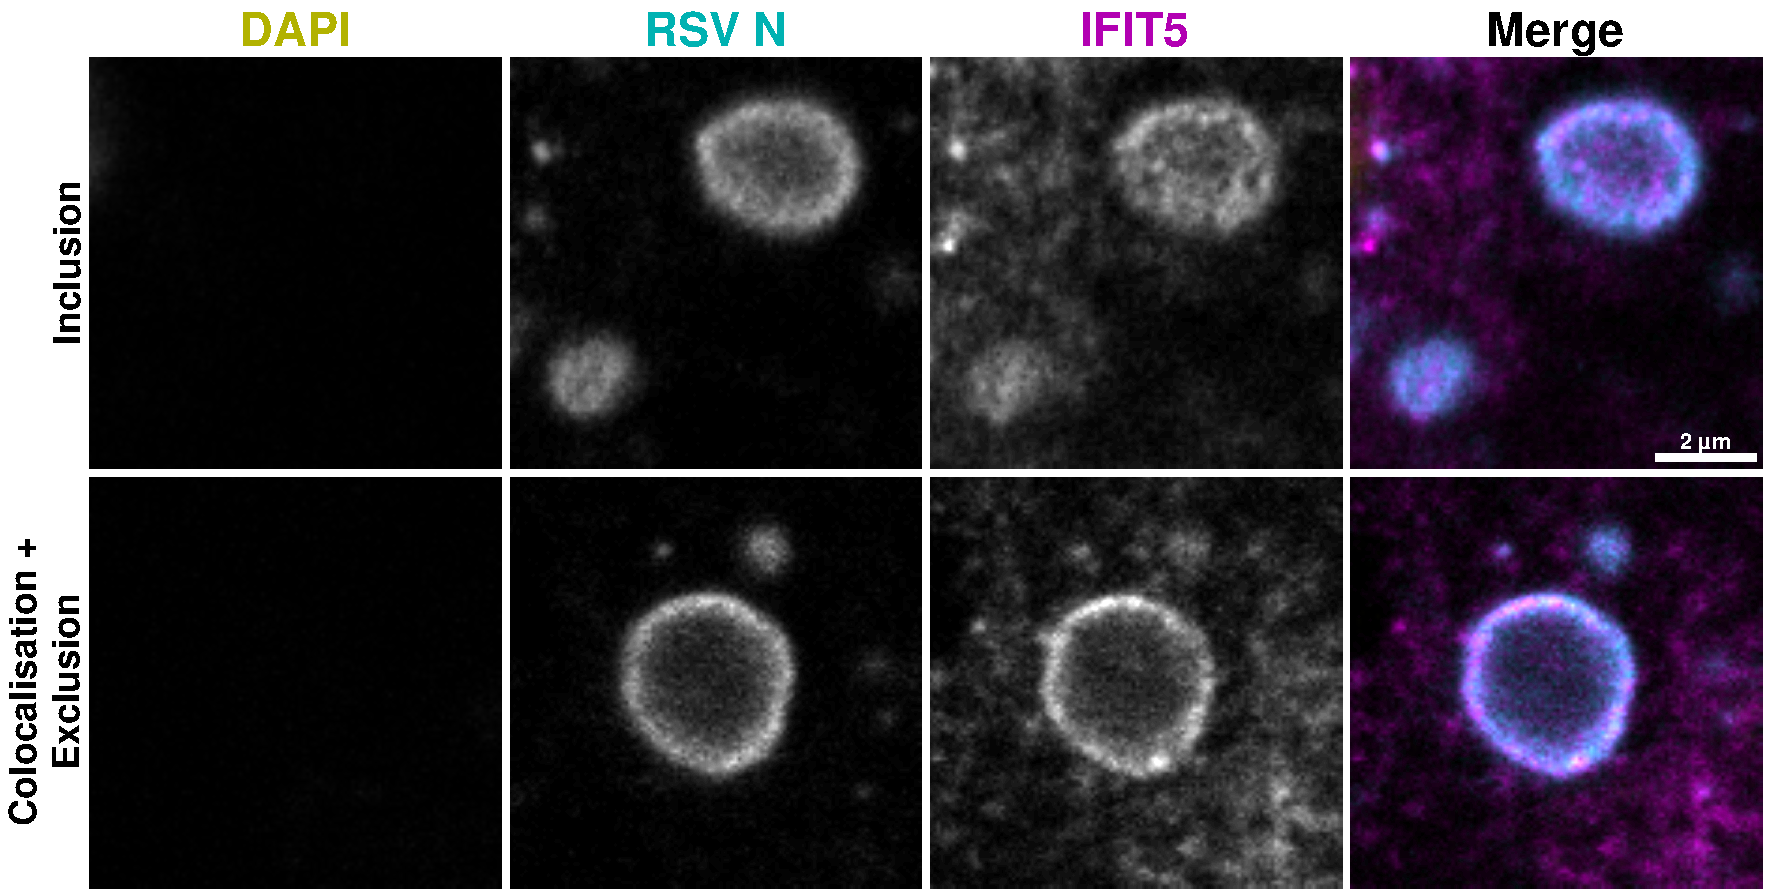
\includegraphics[width=1\linewidth]{09. Chapter 4/Figs/01. pIB/05. IFIT5/03. i5-vero-hnhp.pdf}
    \caption[Representative Images of Interaction Phenotypes of Monkey IFIT5 with Human pIBs in the Vero Cell Line.]{\textbf{Representative Images of Interaction Phenotypes of Monkey IFIT5 with Human pIBs in the Vero Cell Line.} Vero cells were transfected with hRSV N and P containing plasmids using TransIT-X2 and were fixed after 24 hours. Cellular nuclei were stained with DAPI (yellow), and cells were double-labeled with anti-RSV N (cyan) and anti-IFIT5 (magenta) antibodies. This figure showcases representative examples of relevant phenotypes in the interaction between monkey IFIT5 and hRSV pseudo inclusion bodies. These phenotypes are presented in descending order based on their percentage proportions. The scale bar indicates 2 \(\mu \mbox{m}\).}
    \label{fig:Representative Images of Interaction Phenotypes of Monkey IFIT5 with Human pIBs in the VERO Cell Line}
\end{figure}

Finally, we investigated the interactions of IFIT5 with the simplified model of RSV pseudo-inclusion bodies. As previously mentioned, data was exclusively obtained from the Vero cell line transfected with hRSV \textit{N} and \textit{P}-containing plasmids, allowing us to examine the interaction of monkey IFIT5 with human pIBs. Figure \ref{fig:Interaction Phenotypes of Monkey IFIT5 with Human pIBs in the VERO Cell Line} illustrates the frequencies of occurrences of observed phenotypes, along with the measured pIB areas per observed phenotype, based on 100 recorded observations. Representative images of these phenotypes are shown in Figure \ref{fig:Representative Images of Interaction Phenotypes of Monkey IFIT5 with Human pIBs in the VERO Cell Line}. Monkey IFIT5 displayed two hRSV pIB interaction phenotypes, namely forming intra-pIB inclusions (62\% of observations) and colocalising with the pIB boundary while being excluded from the pIB structure (38\% of observations). The size of inclusion-associated hRSV pIBs ranged from 0.13 \(\mu \mbox{m}^2\) to 10 \(\mu \mbox{m}^2\), with an atypical value of 1.2 \(\mu \mbox{m}^2\). Conversely, the size profile of pIBs associated with colocalisation accompanied by exclusion phenotype ranged from 0.23 \(\mu \mbox{m}^2\) to supra 40, with a median value of 4 \(\mu \mbox{m}^2\). Differentiation of these pIBs based on size is apparent, although there is a marked overlap of sizes where both phenotypes occur (between 0.23 and 10 \(\mu \mbox{m}^2\)). Notably, our previous observations indicated minimal interactions of both human and bovine IFIT5 with RSV inclusion bodies during infection, with the most prevalent observed phenotype being exclusion (Chapter \ref{ch:Subcellular Localisation of Endogenous IFIT Proteins in the Context of RSV Inclusion Bodies}). Specifically, we observed the inclusion phenotype in only 10\% of observations in the MDBK cell line and the colocalisation associated with exclusion phenotype in 5\% of observations in the A549 cell line. This suggests that IFIT5 has a propensity to interact with pseudo-inclusion bodies, but factors present in RSV IBs during infection may prevent IFIT5 from accessing these structures.

In summary, the investigation of IFIT1, IFIT3, and IFIT5 localisation in the context of the simplified model of RSV inclusion bodies, using ectopically expressed pseudo-inclusion bodies, yielded intriguing results. These results provide insights into the nature of their interactions and potential factors impeding these interactions during RSV infection. Concerning endogenous IFIT1, minimal interaction was observed in human cells (HEK293T) with hRSV pIBs, although this may be due to a size bias of the observed pIBs. This assumption is based on observed monkey IFIT1 interactions with human RSV pIBs, where strong interaction phenotypes (inclusion and colocalisation) correlated with increased pIB size. This aligns with results from monkey IFIT1 interaction with bovine RSV pIBs, where only phenotypes implying interaction were observed. Monkey IFIT1 data supports observations from Section \ref{subsec:Endogenous IFIT Interaction with RSV Inclusion Bodies}, where both human and bovine IFIT1 showed strong interaction phenotypes (inclusion or colocalisation) with RSV IBs during infection. However, this was not the dominant observed phenotype, which was exclusion. Monkey IFIT3 exhibited data consistent with what was observed in RSV infection data, i.e., the majority of cases being either indirectly associated with pIBs (diffusion) or excluded from the structures, while directly associating with these structures with small but considerable frequency. This suggests that the IFIT3-IB interaction is directed via biophysical interactions with the pIB and IB structures. Finally, monkey IFIT5 showed only strong interaction phenotypes with human pIBs. This is unexpected, as during infection, neither human nor bovine IFIT5 exhibited minimal direct or indirect interaction phenotypes, with the dominant observed phenotype being exclusion. This discrepancy could be due to the differential propensity of monkey IFIT5 for interaction with (p)IBs compared to human and bovine IFIT5, or it could mean that viral or cellular factors associated with and influencing the RSV IBs during infection prevent IFIT5 from interacting with these structures. While these experiments provided valuable data confirming previous observations (as in the case of IFIT3 or IFIT1 interacting with human pIBs), they also yielded inconsistent results with previous observations. Another issue is that the majority of the gathered data is based on monkey IFITs, which are not relevant for human and bovine RSV infection \textit{in vivo}. Thus, it is essential that this data is further validated and investigated using human and bovine IFITs. To achieve this, we aimed to analyze the interaction profiles of exogenously expressed human and bovine IFITs in the context of human and bovine RSV infection.

\subsection{Overexpressed IFIT1, IFIT3, and IFIT5 During RSV Infection} \label{subsec:Overexpressed IFIT1, IFIT3, and IFIT5 During RSV Infection}
In order to validate the interaction results of monkey IFIT1, IFIT3, and IFIT5 with pseudo IBs and to investigate the maximal potential for intereactions between human and bovine IFIT1, IFIT3, and IFIT5 with human and bovine IBs in the context of infection, we further aimed to conduct IFIT overexpression expreiments coupled with RSV infection. We wanted to decrease the likelihood of nonspecific antibody staining by overexpressing FLAG-tagged IFIT proteins, which would be visualised using monoclonal anti-FLAG antibody. The usage of FLAG tag would allow for higher specificity and increased access for IB detection inside of the phase separated structures \cite{Munro1984Use70.}. To do this we needed a library of FLAG-tagged human and bovine IFIT proteins, cloned in plasmids which allow for effcient translation in transfected cells. We were kindly provided with human IFIT1, IFIT2, IFIT3, and IFIT5 ORF-containng plasmids, each tagged with FLAG in the C terminus by the Viral Gene Expressioin group from the Pirbright Institute. This group also provided a control GFP-FLAG pcDNA3.1 plasmid, which was used as a control for transfection efficiency and persistance. These were already present in a  pcDNA3.1 backbone, whcih was directly suitable for our downstream analyses. We were also kindly provided by bovine IFIT-containing plasmids by CVR Glasgow as a part of their bovine ISG plasmid library. There plasmids were consisting of SCRPSY backbone, which is optimasied for creating lentiviral praticles, and untagged bovine IFIT ORFs. Due to this reason we needed to clone these ORF into pcDNA3.1 plasmid backbone, while cocurently adding a C-terminal FLAG tag.

The schematics and decriptions of the pcDNA3.1 and SCRPSY plasmids are depicted in Section \ref{subsec:DNA Plasmids}, while the detailed description of cloning and subcling methodologies are shown in Section \ref{subsec:PCR for Cloning into pcDNA3.1} and Section \ref{subsec:Common Subcloning Methodologies} respectively. Briefly, we have designed forwards and reverse primers, specific for each bovine \textit{IFITs}, consisting of, among other elements, section of the ORF, FLAG tag, start or stop sequence, and the recognition sites of Acc65I and NotI restriction enzymes respectively. These were specificaly selected as their restrictioni sites are not preset within either of the bovine \textit{IFIT} sequence. These primers were used to PCR amplify and isolate the bovine \textit{IFIT} ORFs from the SCRPSY plasmids. These linear ORFs were subsequently subcloned into the pcDNA3.1 plasmid backbones.

To assay the subcellular localisation of exogenously expressed human and bovine IFIT proteins with regards to human and bovine RSV inclusion bodies, we have transfected Vero cells with 1 \(\mu\)g per well of a 24 well plate using TransIT-X2, as decribed in Section \ref{subsec:Transfecting Cells}, and infected the cells with MOI 1 RSV based on the standard methodology (described in Section \ref{subsec:Viral Infections, UV-Inactivation and Ruxolitinib Treatment}). There is an inherent difficulty in establishing cocurrent infection and transfection in the same cells, as doing one treatment usually puts the cell in a antiviral state, that prevents further treatment (infection or transfection). Due to this, we have to tried several methodologies to cause cocurrent infection and transfection. To obtain data that would be comparable with the data previously gathered from infectiion experiments (Chapter \ref{ch:Subcellular Localisation of Endogenous IFIT Proteins in the Context of RSV Inclusion Bodies}) i.e. RSV infection that is terminated 24 HPI, we have initialy tried cell transfection, that was follwed by RSV infection 24 hours post transfection. We used the GFP-FLAG control plasmid to easily assess transfection efficiency and persistance, while we have examined the cells for RSV cytophatic effect (e.g. syncytia formation) to confirm sucessful infection. While we were able to detect sucesful transfection 24 hours post transfection, after 24 hours of subvsequent infection none GFP-expression was detected. Next, we have tried simultanoues infection and transfection. This was done by initial inoculatyion of the cells with a virus preparation and incubation with this innoculum for an hour. Afterwards the inoculum was removed, the cells washed with PBS, after which the trabsfection mixture was added in the cell culture media. This however also resulted in minimal GFP expression. In both of these methodologies we have observed robust infection. Lastly we have emplyed initial RSV infection, followed by transfection 24 HPI. The cells were fixed 24 hours post transfection i.e. 48 hours post infection. This methogology yielded the best co-infection/transfection out of all methodologies tried. Saying this, it was still sub optimal as for some IFIT/RSV conbinations we have only detected 10-15 co-infection/transfection cells, although sufficient for confocal microscopy analysis.

This is to be expected as we know that overexpressed hIFIT1, hIFIT2, and hIFIT3 are antiviral against RSV and thus cells that would present ectopicaly expressded IFITs would therefore create an enviroment that would be unbsuitable for RSV life cycle. Along to this and as mantioned above, infected cells activate their innate antiviral pahtwasys and thus prevent another infection or transfection. This creates inherent bias whereby the cells which have the propensity to be coccurently infected and transfected are not representative of the general cellular population. With regards to the lenght of the infection, after 48 HPI we can expect the size of the IBs to be substantialy larger to what we observed at 24 HPI previously. It is reported in the literature that the mean 2D area of bRSV incusion bodies increased from 8.99 \(\mu \mbox{m}^2\) to 22.18 \(\mu \mbox{m}^2\) between 24 HPI and 48 HPI \cite{Jobe2021BovineResponses}. This would thus make it difficult to compare the co-infection/transfection data to the infection data from Chapter \ref{ch:Subcellular Localisation of Endogenous IFIT Proteins in the Context of RSV Inclusion Bodies}. We could however use the present data to investigate the potential influence of ectopicaly expressed IFIT proteins on the 2D IB area, which could be used to gauge the potential anti-RSV mechanism of these proteins. We experienced difficulties in obtaining co-infection/transfection data with several plasmids. These include bovine IFIT1, human IFIT3, and bovine IFIT5. These were possibly die to a variety of reasons e.g. decreased teransfection efficiency due to contaminats present in the plasmid preparation or the tranfection complexex failing to form properly. All of the data presented below is supported by z-stack measurements.

\begin{figure}
    \begin{subfigure}{0.495\textwidth}
        \caption{}
        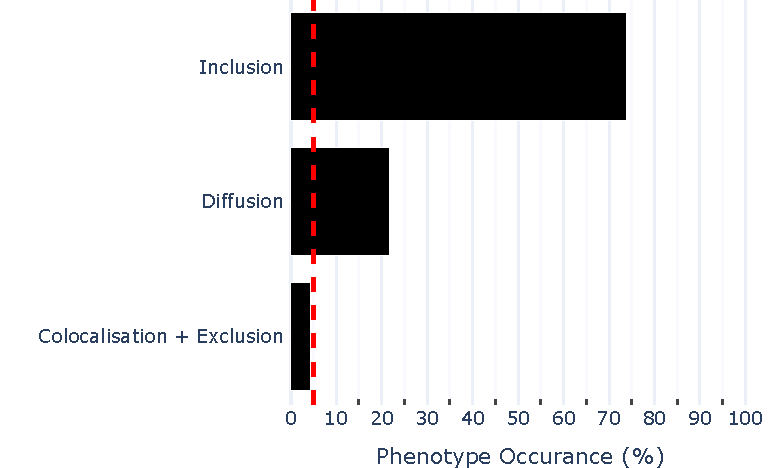
\includegraphics[width=1\linewidth]{09. Chapter 4/Figs/02. Overexpression/01. IFIT1/01. bar_i1_hrsv.pdf} 
    \end{subfigure}
    \begin{subfigure}{0.495\textwidth}
        \caption{}
        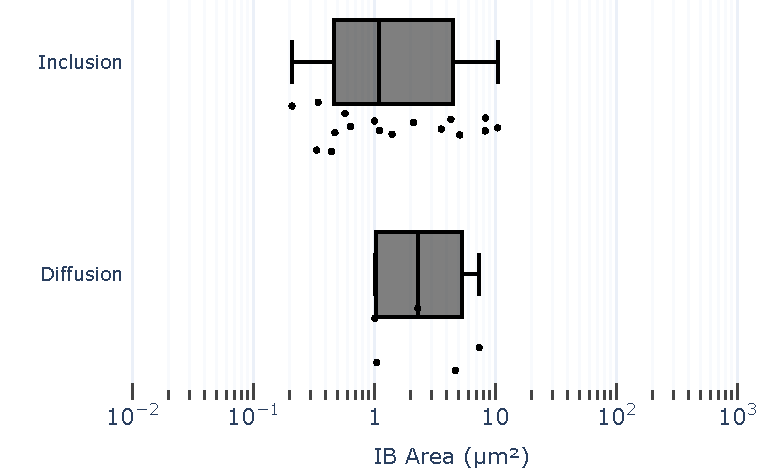
\includegraphics[width=1\linewidth]{09. Chapter 4/Figs/02. Overexpression/01. IFIT1/02. box_i1_hrsv.pdf}
    \end{subfigure}
    \caption[Observed Phenotypes of Exogenous hIFIT1 in the Context of hRSV Inclusion Bodies in Vero Cell Line.]{\textbf{Observed Phenotypes of Exogenous hIFIT1 in the Context of hRSV Inclusion Bodies in Vero Cell Line.} Vero cells were infected with human RSV at MOI 1. 24 HPI, the cells were transfected with hIFIT1-FLAG containing plasmids using TransIT-X2 and were fixed after a further 24 hours. Cells were labelled with anti-RSV N and anti-FLAG antibodies and imaged on a confocal microscope. Panel (a) shows the percentual proportions of observed phenotypes between hRSV inclusion bodies and exogenous hIFIT1 (23 observations), with the red dotted line denoting the 5\% threshold, marking phenotypes considered relevant above this limit. Panel (b) shows the IB area in \(\mu \mbox{m}^2\) per observed relevant phenotype.}
    \label{fig:Observed Phenotypes of Exogenous hIFIT1 in the Context of hRSV Inclusion Bodies in VERO Cell Line}
\end{figure}

\begin{figure}
    \centering
    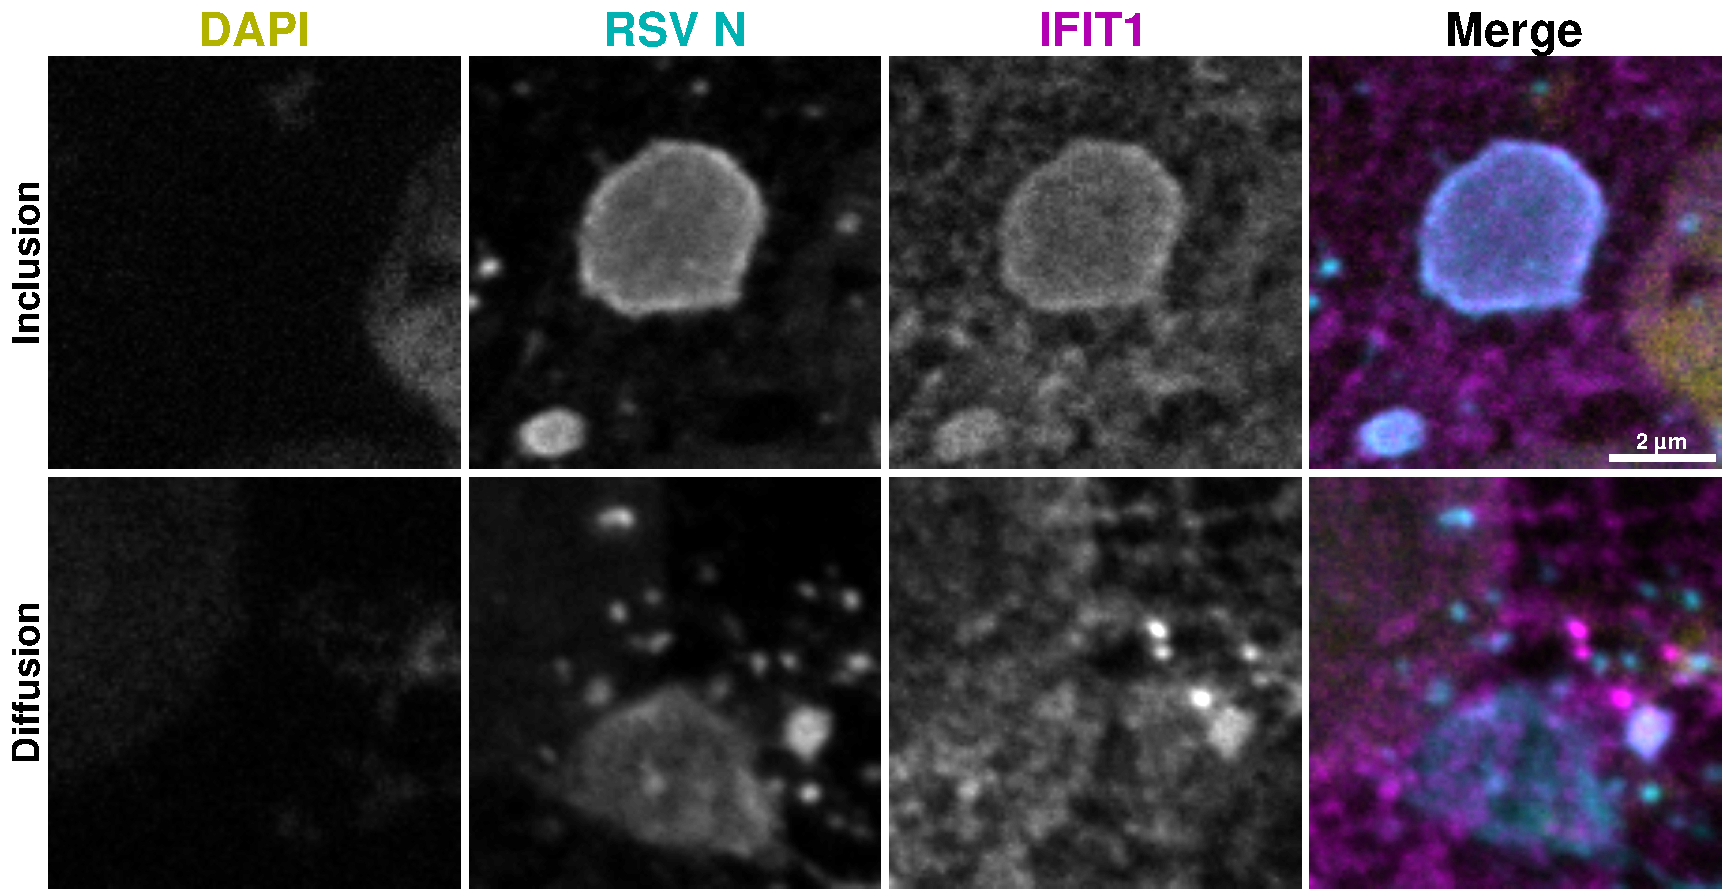
\includegraphics[width=1\linewidth]{09. Chapter 4/Figs/02. Overexpression/01. IFIT1/03. i1-hrsv.pdf}
    \caption[Representative Images of Observed Phenotypes of Exogenous hIFIT1 in the Context of hRSV Inclusion Bodies in Vero Cell Line.]{\textbf{Representative Images of Observed Phenotypes of Exogenous hIFIT1 in the Context of hRSV Inclusion Bodies in Vero Cell Line.} Vero cells were infected with human RSV at MOI 1. 24 HPI, the cells were transfected with hIFIT1-FLAG containing plasmids using TransIT-X2 and were fixed after a further 24 hours. Cellular nuclei were stained with DAPI (yellow), and cells were double-labelled with anti-RSV N (cyan) and anti-FLAG (magenta) antibodies. This figure showcases representative examples of relevant phenotypes in the interaction between exogenous hIFIT1 and hRSV inclusion bodies. These phenotypes are presented in descending order based on their percentage proportions. The scale bar indicates 2 \(\mu \mbox{m}\).}
    \label{fig:Representative Images of Observed Phenotypes of Exogenous hIFIT1 in the Context of hRSV Inclusion Bodies in VERO Cell Line}
\end{figure}

We have observed 23 instances of human IFIT1 being expressed in hRSV infected cells. The frequencies of occurances of observed phenotypes along to the measured IB sizes of phenotypes occuring with >5\% fruequency are shown in Figure \ref{fig:Observed Phenotypes of Exogenous hIFIT1 in the Context of hRSV Inclusion Bodies in VERO Cell Line}. The representative images of the latter are shown in Figure \ref{fig:Representative Images of Observed Phenotypes of Exogenous hIFIT1 in the Context of hRSV Inclusion Bodies in VERO Cell Line}. The most commonly occurng phenotype was intra-IB inclusion, which was observed in 74\% of observations. This was followed by a diffusioin phenotype (22\%), and colocalisation associated with IB exclusion (4\%). Since the latter occured in sub 5\% frequency it was exluded from the size analysis. With regards to the size of inclusion phenotype-associated IBs, they encompasses the whole size spectrum of the IBs observed in this condition (i.e. hIFIT1 and hRSV co-infection/transfection) ranging from 0.2 \(\mu \mbox{m}^2\) to 10 \(\mu \mbox{m}^2\), with the typical size of 1.1 \(\mu \mbox{m}^2\). The diffusion-associated IBs were observed to be between 1 \(\mu \mbox{m}^2\) and 7 \(\mu \mbox{m}^2\) in size, with the median value of 2.2 \(\mu \mbox{m}^2\). This shows that small sub 1 \(\mu \mbox{m}^2\) IBs specificaly present inclusion phenotyoe while the medium sized IBs dyspolay both inclusion and diffusion phenotypes. Interestiingly we have not observed IBs larger than 10 \(\mu \mbox{m}^2\), which is unusual for for IBs observed at 48 HPI. The reason could be the anti RSV action of hIFIT1.

\begin{figure}
    \begin{subfigure}{0.495\textwidth}
        \caption{}
        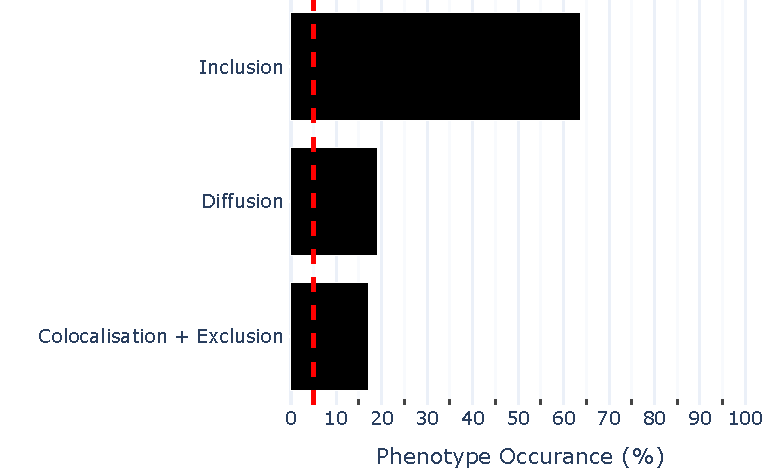
\includegraphics[width=1\linewidth]{09. Chapter 4/Figs/02. Overexpression/01. IFIT1/04. bar_i1_brsv.pdf} 
    \end{subfigure}
    \begin{subfigure}{0.495\textwidth}
        \caption{}
        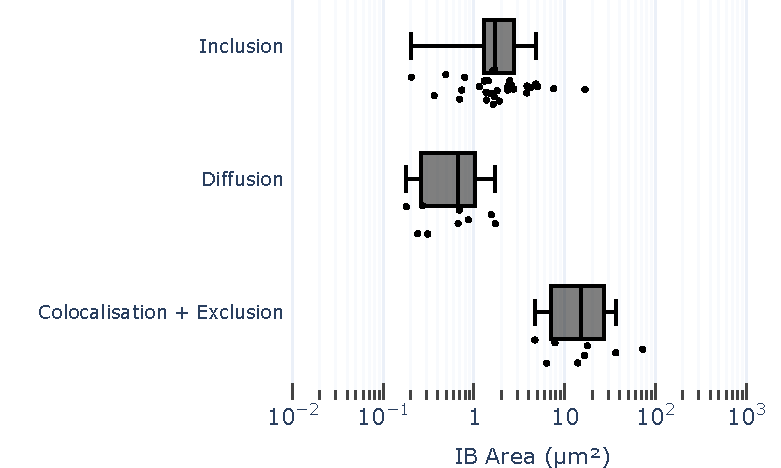
\includegraphics[width=1\linewidth]{09. Chapter 4/Figs/02. Overexpression/01. IFIT1/05. box_i1_brsv.pdf}
    \end{subfigure}
    \caption[Observed Phenotypes of Exogenous hIFIT1 in the Context of bRSV Inclusion Bodies in Vero Cell Line.]{\textbf{Observed Phenotypes of Exogenous hIFIT1 in the Context of bRSV Inclusion Bodies in Vero Cell Line.} Vero cells were infected with bovine RSV at MOI 1. 24 HPI, the cells were transfected with hIFIT1-FLAG containing plasmids using TransIT-X2 and were fixed after further 24 hours. Cells were labeled with anti-RSV N and anti-FLAG antibodies and imaged on confocal microscope. Panel (a) shows percentual proportions of observed phenotypes between bRSV inclusion bodies and exogenous hIFIT1 (47 observations), with the red dotted line denoting the 5\% threshold, marking phenotypes considered relevant above this limit. Panel (b) shows the IB area in \(\mu \mbox{m}^2\) per observed relevant phenotype.}
    \label{fig:Observed Phenotypes of Exogenous hIFIT1 in the Context of bRSV Inclusion Bodies in VERO Cell Line}
\end{figure}

\begin{figure}
    \centering
    \includegraphics[width=1\linewidth]{09. Chapter 4/Figs/02. Overexpression/01. IFIT1/06. i1-brsv.pdf}
    \caption[Representative Images of Observed Phenotypes of Exogenous hIFIT1 in the Context of bRSV Inclusion Bodies in Vero Cell Line.]{\textbf{Representative Images of Observed Phenotypes of Exogenous hIFIT1 in the Context of bRSV Inclusion Bodies in Vero Cell Line.} Vero cells were infected with bovine RSV at MOI 1. 24 HPI, the cells were transfected with hIFIT1-FLAG containing plasmids using TransIT-X2 and were fixed after further 24 hours. Cellular nuclei were stained with DAPI (yellow), and cells were double-labeled with anti-RSV N (cyan) and anti-FLAG (magenta) antibodies. This figure showcases representative examples of relevant phenotypes in the interaction between exogenous hIFIT1 and bRSV inclusion bodies. These phenotypes are presented in descending order based on their percentage proportions. The scale bar indicates 2 \(\mu \mbox{m}\).}
    \label{fig:Representative Images of Observed Phenotypes of Exogenous hIFIT1 in the Context of bRSV Inclusion Bodies in VERO Cell Line}
\end{figure}

Next we intestigated the interaction of ectopicaly expressed human IFIT1 with regards to bRSV incusion bodies. We have obtained 47 observation. The frequencies of occurance of the observed phenotypes alonbg with the measured IB sizes per associated phenotypes are shown in Figure \ref{fig:Observed Phenotypes of Exogenous hIFIT1 in the Context of bRSV Inclusion Bodies in VERO Cell Line}. The representative images are shown in Figure \ref{fig:Representative Images of Observed Phenotypes of Exogenous hIFIT1 in the Context of bRSV Inclusion Bodies in VERO Cell Line}. We have observed identical phenotypes to what was observed during hRSv infection, with almost the identical frequencies of occurance. The most common interaction phenotype was inclusion, which occured in 64\% of observations. This was followed by the diffusion and colocalisation associated wth intra IB exclusiion, which occured at 19\% and 16\% respectively. We see a relatvely well diferensiation of the observed phenotypes based on the observed IB areas. Although the incluson-phenotype associated IB areas ranged from 0.2 \(\mu \mbox{m}^2\) to supra 10 \(\mu \mbox{m}^2\) with a typical size of 1.8 \(\mu \mbox{m}^2\), most of the IBs associated with this phenotype custered between 1 and 5 \(\mu \mbox{m}^2\). The diffusion phgenotype occured in smaller IBs which ranged from sub 0.2 \(\mu \mbox{m}^2\) to supra 1 \(\mu \mbox{m}^2\), wth the median size of 0.8 \(\mu \mbox{m}^2\). Lastly, the colocalisation associated with excluson was observed only in large and very large IBs, which size ranged from sub 5 \(\mu \mbox{m}^2\) to 70 \(\mu \mbox{m}^2\), with the median size of 14 \(\mu \mbox{m}^2\). Clearly there is a size separation between the IB association with either diffusion (small IBs) or colocalsation acompanied with exclusion (large IBs) phenotypes. The inclusion phenotype was most comonly observed in the IBs with the size between these two groups, although it was observed in extremely sized IBs from both sides. This differenation could be as a result of differential maturation status of the incusion bodies. It is possible that newly formed small IBs are initially IFIT1-less, although IFIT1 has access to these structures. Afterwards IFIT1 associates and concentrates inside these scructures. As they mature and increase in size and complexity, as well as become more gel like, IFIT1 transclocate to the periphery of the IB.

\begin{figure}
    \begin{subfigure}{0.495\textwidth}
        \caption{}
        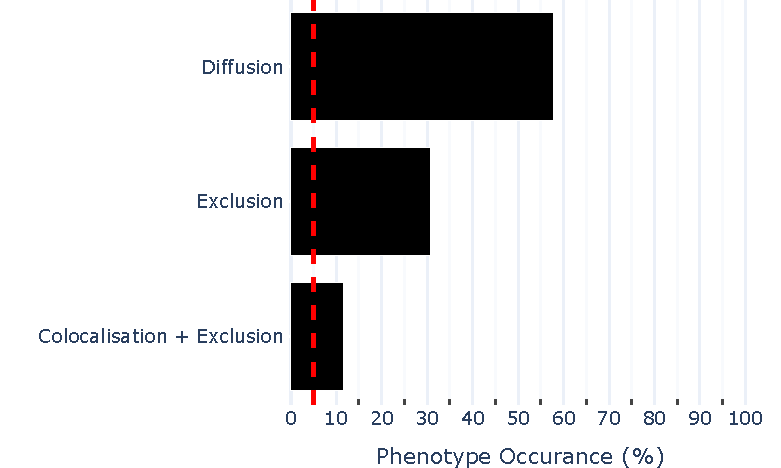
\includegraphics[width=1\linewidth]{09. Chapter 4/Figs/02. Overexpression/03. IFIT3/01. bar_i3_hrsv.pdf} 
    \end{subfigure}
    \begin{subfigure}{0.495\textwidth}
        \caption{}
        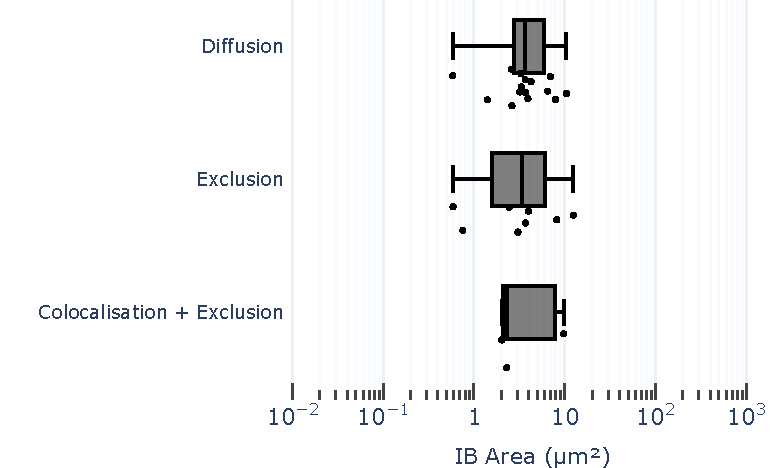
\includegraphics[width=1\linewidth]{09. Chapter 4/Figs/02. Overexpression/03. IFIT3/02. box_i3_hrsv.pdf}
    \end{subfigure}
    \caption[Observed Phenotypes of Exogenous bIFIT3 in the Context of hRSV Inclusion Bodies in Vero Cell Line.]{\textbf{Observed Phenotypes of Exogenous bIFIT3 in the Context of hRSV Inclusion Bodies in Vero Cell Line.} Vero cells were infected with human RSV at MOI 1. 24 HPI, the cells were transfected with bIFIT3-FLAG containing plasmids using TransIT-X2 and were fixed after further 24 hours. Cells were labeled with anti-RSV N and anti-FLAG antibodies and imaged on confocal microscope. Panel (a) shows percentual proportions of observed phenotypes between hRSV inclusion bodies and exogenous bIFIT3 (26 observations), with the red dotted line denoting the 5\% threshold, marking phenotypes considered relevant above this limit. Panel (b) shows the IB area in \(\mu \mbox{m}^2\) per observed relevant phenotype.}
    \label{fig:Observed Phenotypes of Exogenous bIFIT3 in the Context of hRSV Inclusion Bodies in VERO Cell Line}
\end{figure}

\begin{figure}
    \centering
    \includegraphics[width=1\linewidth]{09. Chapter 4/Figs/02. Overexpression/03. IFIT3/03. bi3-hrsv.pdf}
    \caption[Representative Images of Observed Phenotypes of Exogenous bIFIT3 in the Context of hRSV Inclusion Bodies in Vero Cell Line.]{\textbf{Representative Images of Observed Phenotypes of Exogenous bIFIT3 in the Context of hRSV Inclusion Bodies in Vero Cell Line.} Vero cells were infected with human RSV at MOI 1. 24 HPI, the cells were transfected with bIFIT3-FLAG containing plasmids using TransIT-X2 and were fixed after further 24 hours. Cellular nuclei were stained with DAPI (yellow), and cells were double-labeled with anti-RSV N (cyan) and anti-FLAG (magenta) antibodies. This figure showcases representative examples of relevant phenotypes in the interaction between exogenous bIFIT3 and hRSV inclusion bodies. These phenotypes are presented in descending order based on their percentage proportions. The scale bar indicates 2 \(\mu \mbox{m}\).}
    \label{fig:Representative Images of Observed Phenotypes of Exogenous bIFIT3 in the Context of hRSV Inclusion Bodies in VERO Cell Line}
\end{figure}

Next we set to nvestiigate the exogenous bovine IFIT3 intrreaction with hRSV IBs. Within 26 total observations we have identified 3 intreraction phenotypes, all of which occured above 5\% frequency. The respective phenotypes, ther frequences along with the mearured 2D area of the IBs is shown in Figure \ref{fig:Observed Phenotypes of Exogenous bIFIT3 in the Context of hRSV Inclusion Bodies in VERO Cell Line}. The representative images of these phenotypes are shown in Figure \ref{fig:Representative Images of Observed Phenotypes of Exogenous bIFIT3 in the Context of hRSV Inclusion Bodies in VERO Cell Line}. Unlike what we observed with human IFIT1, the predominant phenotypes do not imply interaction. The most comonly observed phenotype was diffusion (57\%), followed by exclusion (31\%), and colocalisaion associated with intra-IB exclusion (12\%). Although showing minute diffrences in the median observed IB sizes, all phenotypes were associated with almost identicaly sized IBs. In more detail diffusion-associated IBs ranged in size from 0.6 \(\mu \mbox{m}^2\) to supra 10 \(\mu \mbox{m}^2\), with the median value of 4 \(\mu \mbox{m}^2\). The size of exclusion-associated IBs also ranged from 0.6 \(\mu \mbox{m}^2\) to supra 10 \(\mu \mbox{m}^2\), but showed a typical value of 3.3 \(\mu \mbox{m}^2\). Lastly, the colocalisation associated with exclusion was observed to be associated with 3 IBs, which had sizes of 2 \(\mu \mbox{m}^2\), 2.1 \(\mu \mbox{m}^2\), and 10 \(\mu \mbox{m}^2\). This data suggest that these phenotypes occur independently of IB maturity. Interestingly we have failed to observe IBs with 2D areas above 10 \(\mu \mbox{m}^2\). This could be due to the the limited number of observations. It could also be explained by seemingly IB-intreaction independent anti-RSV action of bovine IFIT3, which limits the maximum size these structures can be.

\begin{figure}
    \begin{subfigure}{0.495\textwidth}
        \caption{}
        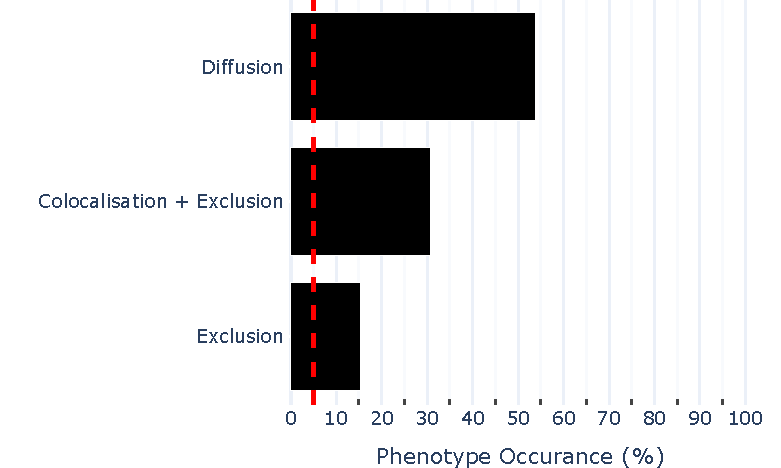
\includegraphics[width=1\linewidth]{09. Chapter 4/Figs/02. Overexpression/03. IFIT3/04. bar_i3_brsv.pdf} 
    \end{subfigure}
    \begin{subfigure}{0.495\textwidth}
        \caption{}
        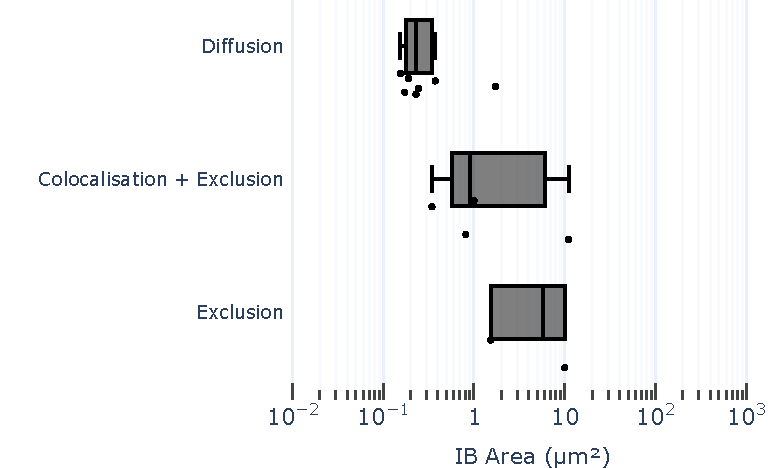
\includegraphics[width=1\linewidth]{09. Chapter 4/Figs/02. Overexpression/03. IFIT3/05. box_i3_brsv.pdf}
    \end{subfigure}
    \caption[Observed Phenotypes of Exogenous bIFIT3 in the Context of bRSV Inclusion Bodies in Vero Cell Line.]{\textbf{Observed Phenotypes of Exogenous bIFIT3 in the Context of bRSV Inclusion Bodies in Vero Cell Line.} Vero cells were infected with bovine RSV at MOI 1. 24 HPI, the cells were transfected with bIFIT3-FLAG containing plasmids using TransIT-X2 and were fixed after further 24 hours. Cells were labeled with anti-RSV N and anti-FLAG antibodies and imaged on confocal microscope. Panel (a) shows percentual proportions of observed phenotypes between bRSV inclusion bodies and exogenous bIFIT3 (13 observations), with the red dotted line denoting the 5\% threshold, marking phenotypes considered relevant above this limit. Panel (b) shows the IB area in \(\mu \mbox{m}^2\) per observed relevant phenotype.}
    \label{fig:Observed Phenotypes of Exogenous bIFIT3 in the Context of bRSV Inclusion Bodies in VERO Cell Line}
\end{figure}

\begin{figure}
    \centering
    \includegraphics[width=1\linewidth]{09. Chapter 4/Figs/02. Overexpression/03. IFIT3/06. bi3-brsv.pdf}
    \caption[Representative Images of Observed Phenotypes of Exogenous bIFIT3 in the Context of bRSV Inclusion Bodies in Vero Cell Line.]{\textbf{Representative Images of Observed Phenotypes of Exogenous bIFIT3 in the Context of bRSV Inclusion Bodies in Vero Cell Line.} Vero cells were infected with bovine RSV at MOI 1. 24 HPI, the cells were transfected with bIFIT3-FLAG containing plasmids using TransIT-X2 and were fixed after further 24 hours. Cellular nuclei were stained with DAPI (yellow), and cells were double-labeled with anti-RSV N (cyan) and anti-FLAG (magenta) antibodies. This figure showcases representative examples of relevant phenotypes in the interaction between exogenous bIFIT3 and bRSV inclusion bodies. These phenotypes are presented in descending order based on their percentage proportions. The scale bar indicates 2 \(\mu \mbox{m}\).}
    \label{fig:Representative Images of Observed Phenotypes of Exogenous bIFIT3 in the Context of bRSV Inclusion Bodies in VERO Cell Line}
\end{figure}

To validate the previous data and to establish if the seemingly non interactive nature of bovine IFIT3 with human IBs is due to the species difference we have set to investigate the interaction phenotypes between ectopicaly expressed bovine IFIT3 bRSV IBs. We obtained only 13 observations in ths analysis. The observed phenotypes along with their frequencies of occurance along with the IB sizes are shown in Figure \ref{fig:Observed Phenotypes of Exogenous bIFIT3 in the Context of bRSV Inclusion Bodies in VERO Cell Line}. The representative images of these phenotypes are shown in Figure \ref{fig:Representative Images of Observed Phenotypes of Exogenous bIFIT3 in the Context of bRSV Inclusion Bodies in VERO Cell Line}. In 54\% of observations we have observed bovine IFIT3 to be diffused throught the bRSV IBs. This was followed by colocalisation acompanied with excluision (31\%) and excluson (15\%) phenotypes. Unlike what was observed when we investigated the interaction of exogenous bIFIT3 with hRSV IBs, there seems to be a size distinction of IBs associated with the different phenotypes. The diffusion phenotype was observed predominantly in very small IBs, which size ranged from sub 0.2 \(\mu \mbox{m}^2\) to sub 2 \(\mu \mbox{m}^2\), with the median value of 0.9 \(\mu \mbox{m}^2\)where most of the IBs clustered. bIFIT3 was observed to colocalise with IB edge while beng excluded from ther centre of these structures in IBs with median size of 0.9 \(\mu \mbox{m}^2\). Lastly, the exclusion phenotype was associated with two IBs of sizes of 1.5 \(\mu \mbox{m}^2\) and 10 \(\mu \mbox{m}^2\). It is to be noted that the population of observed IBs is of a smaller size and we have failed to observe IBs with area larger than 10 \(\mu \mbox{m}^2\), which is unusual for 48 HPI RSV infection. This could be atreributed to the overall small amount of observations or to the potential IB interction-independent anti-RSV action of bovine IFIT3.

\begin{figure}
    \begin{subfigure}{0.495\textwidth}
        \caption{}
        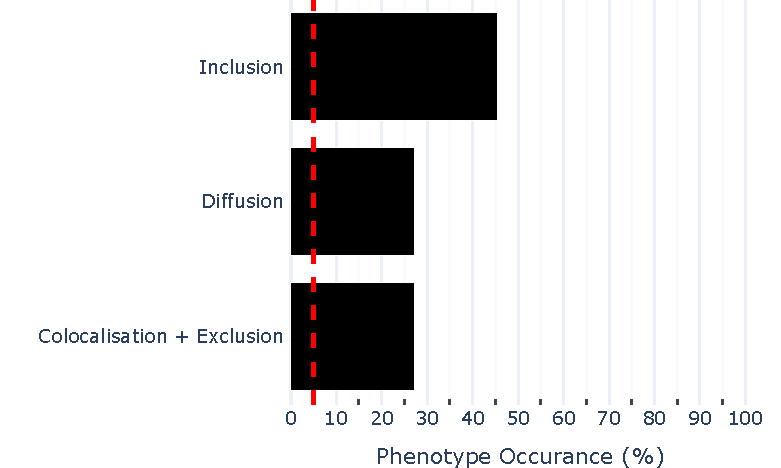
\includegraphics[width=1\linewidth]{09. Chapter 4/Figs/02. Overexpression/04. IFIT5/01. bar_i5_hrsv.pdf} 
    \end{subfigure}
    \begin{subfigure}{0.495\textwidth}
        \caption{}
        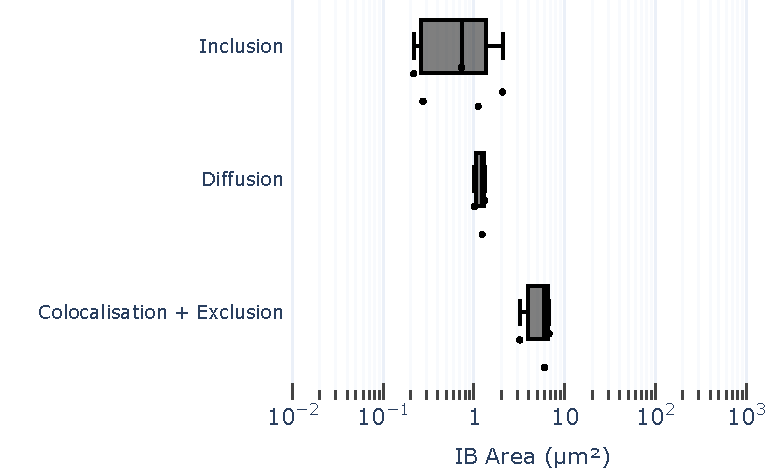
\includegraphics[width=1\linewidth]{09. Chapter 4/Figs/02. Overexpression/04. IFIT5/02. box_i5_hrsv.pdf}
    \end{subfigure}
    \caption[Observed Phenotypes of Exogenous hIFIT5 in the Context of hRSV Inclusion Bodies in Vero Cell Line.]{\textbf{Observed Phenotypes of Exogenous hIFIT5 in the Context of hRSV Inclusion Bodies in Vero Cell Line.} Vero cells were infected with human RSV at MOI 1. 24 HPI, the cells were transfected with hIFIT5-FLAG containing plasmids using TransIT-X2 and were fixed after further 24 hours. Cells were labeled with anti-RSV N and anti-FLAG antibodies and imaged on confocal microscope. Panel (a) shows percentual proportions of observed phenotypes between hRSV inclusion bodies and exogenous hIFIT5 (11 observations), with the red dotted line denoting the 5\% threshold, marking phenotypes considered relevant above this limit. Panel (b) shows the IB area in \(\mu \mbox{m}^2\) per observed relevant phenotype.}
    \label{fig:Observed Phenotypes of Exogenous hIFIT5 in the Context of hRSV Inclusion Bodies in VERO Cell Line}
\end{figure}

\begin{figure}
    \centering
    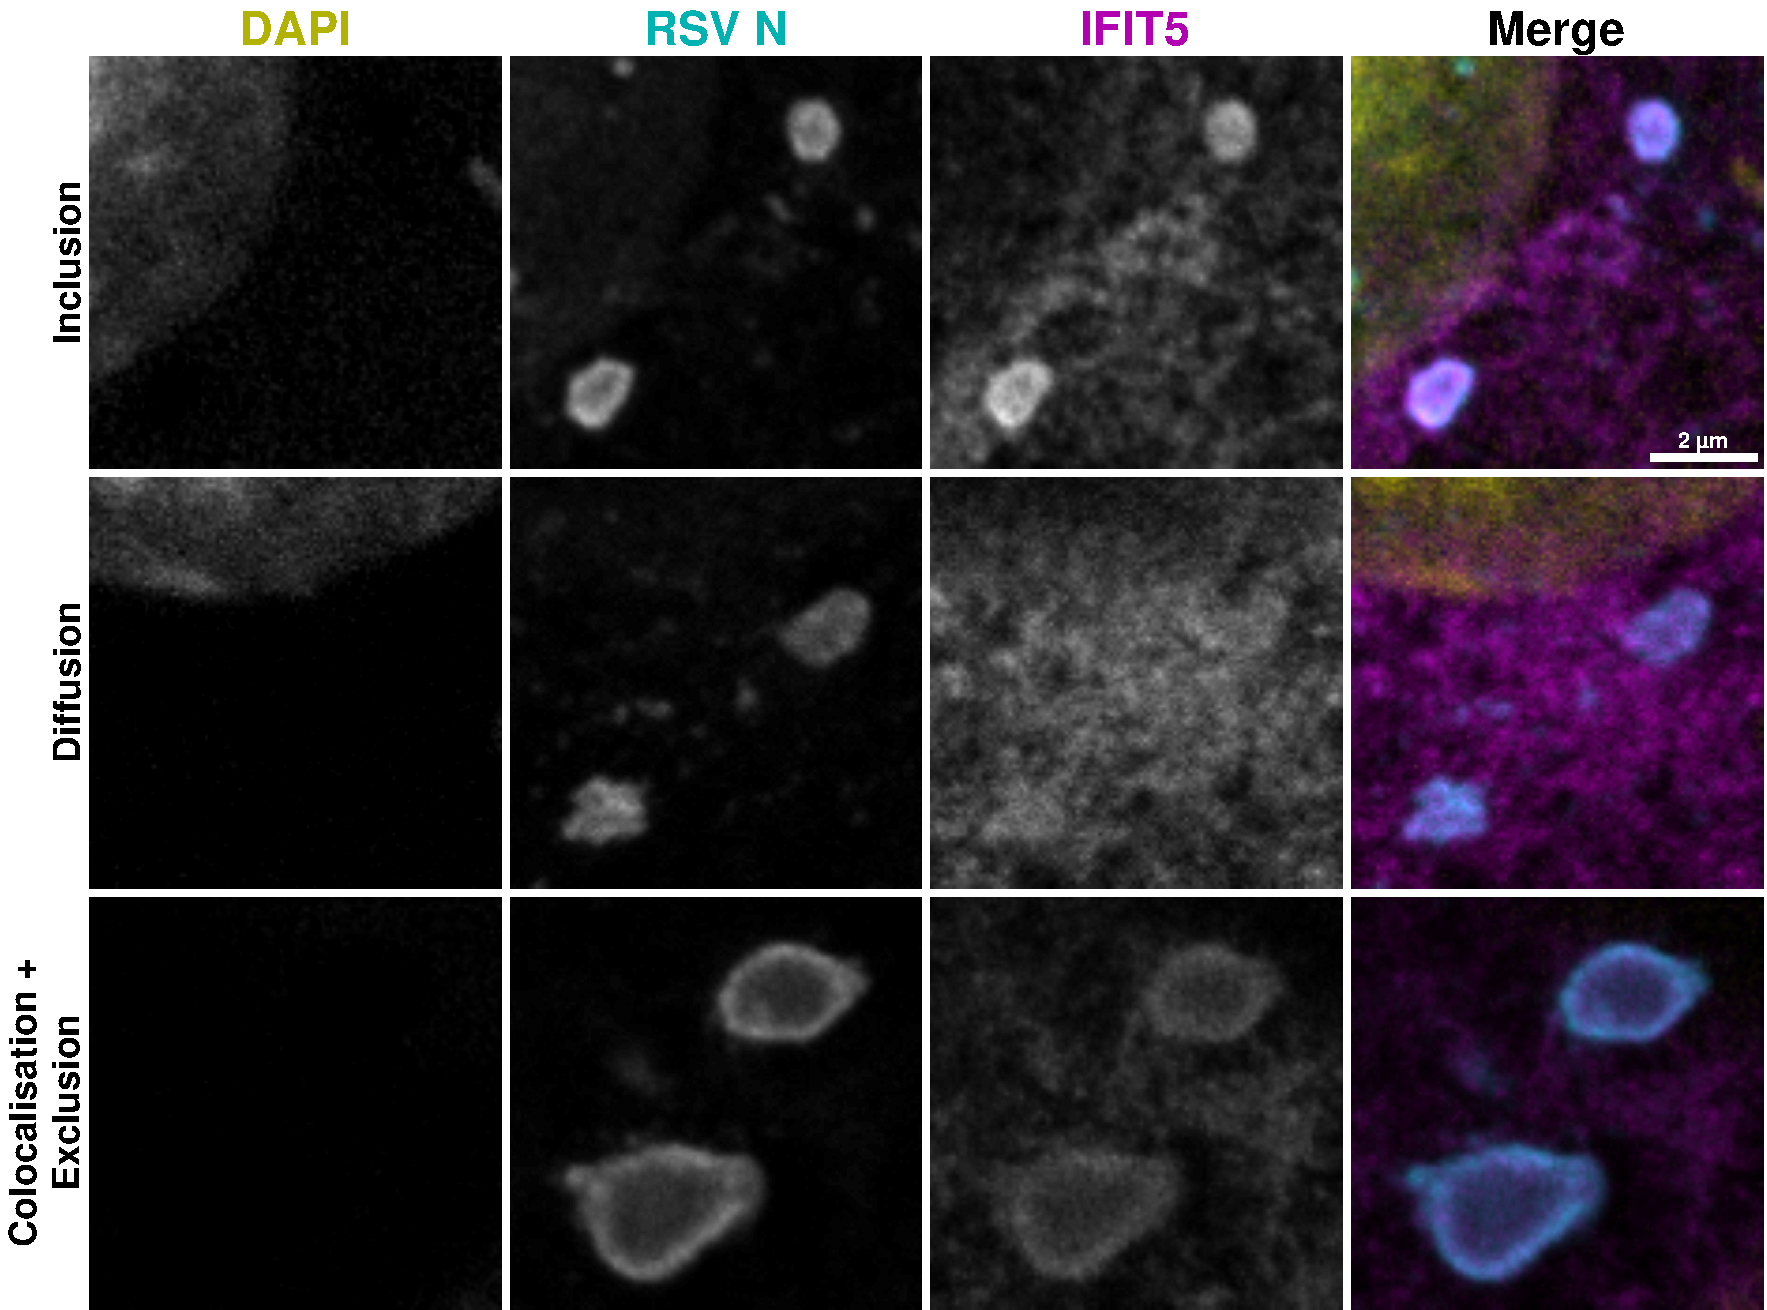
\includegraphics[width=1\linewidth]{09. Chapter 4/Figs/02. Overexpression/04. IFIT5/03. i5-hrsv.pdf}
    \caption[Representative Images of Observed Phenotypes of Exogenous hIFIT5 in the Context of hRSV Inclusion Bodies in Vero Cell Line.]{\textbf{Representative Images of Observed Phenotypes of Exogenous hIFIT5 in the Context of hRSV Inclusion Bodies in Vero Cell Line.} Vero cells were infected with human RSV at MOI 1. 24 HPI, the cells were transfected with hIFIT5-FLAG containing plasmids using TransIT-X2 and were fixed after further 24 hours. Cellular nuclei were stained with DAPI (yellow), and cells were double-labeled with anti-RSV N (cyan) and anti-FLAG (magenta) antibodies. This figure showcases representative examples of relevant phenotypes in the interaction between exogenous hIFIT5 and hRSV inclusion bodies. These phenotypes are presented in descending order based on their percentage proportions. The scale bar indicates 2 \(\mu \mbox{m}\).}
    \label{fig:Representative Images of Observed Phenotypes of Exogenous hIFIT5 in the Context of hRSV Inclusion Bodies in VERO Cell Line}
\end{figure}

Lastly we investigated the interaction of exogenously expressed human IFIT5 with hRSV IBs. We have collected 11 observations which showed 3 interaction phenotypes. These and their associated frequencies of occurances along with the measured IB sizes can be viewed in Figure \ref{fig:Observed Phenotypes of Exogenous hIFIT5 in the Context of hRSV Inclusion Bodies in VERO Cell Line}. The representative images of these phenotypes are shown in Figure \ref{fig:Representative Images of Observed Phenotypes of Exogenous hIFIT5 in the Context of hRSV Inclusion Bodies in VERO Cell Line}. The most comonly observed intreaction phenotype was intra-IB inclusion, which occured in 45\% of observations. This was followed by diffusion and colocalisation associated with exclusoion phenotypes, both of which accured in 26\% of observations. The inclusion phenotype occured in relatively small IBs, which ranged from sub 0.2 \(\mu \mbox{m}^2\) to 2 \(\mu \mbox{m}^2\) in size, with the median value of 0.7 \(\mu \mbox{m}^2\). The diffusion associated IBs toghtly clustered around their median size of 1.2 \(\mu \mbox{m}^2\). Lastly, the colocalisation associated with exclusion phenotype-associated IBs were larger in size, with a typical size of 6 \(\mu \mbox{m}^2\). It is evident that there is IB size-dependentr discintion of phenotypes. In small, sub 1 \(\mu \mbox{m}^2\) IBs human IFIT5 concentrates withing these structures. Asd the IBs increase in size and mature, the inclusion phenotype is maintaned, but also accompanied by diffusion phenotype. Lastly as the IBs further increase in size and reach the limt where IBAGs were reported to occur form the literature, human IFIT5 translocate from the IB interior to the IB boundry. It is to be noted that we have not observed IBs above 7 \(\mu \mbox{m}^2\) in size, suggesting yet again that we are dealing with a incomplete dataset or the increased concentraton of IFIT5 prevents larger IBs from forming.

\begin{figure}
    \begin{subfigure}{0.495\textwidth}
        \caption{}
        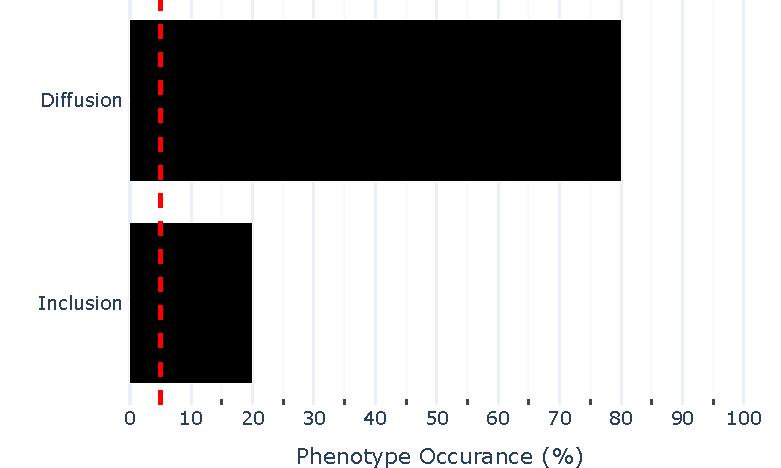
\includegraphics[width=1\linewidth]{09. Chapter 4/Figs/02. Overexpression/04. IFIT5/04. bar_i5_brsv.pdf} 
    \end{subfigure}
    \begin{subfigure}{0.495\textwidth}
        \caption{}
        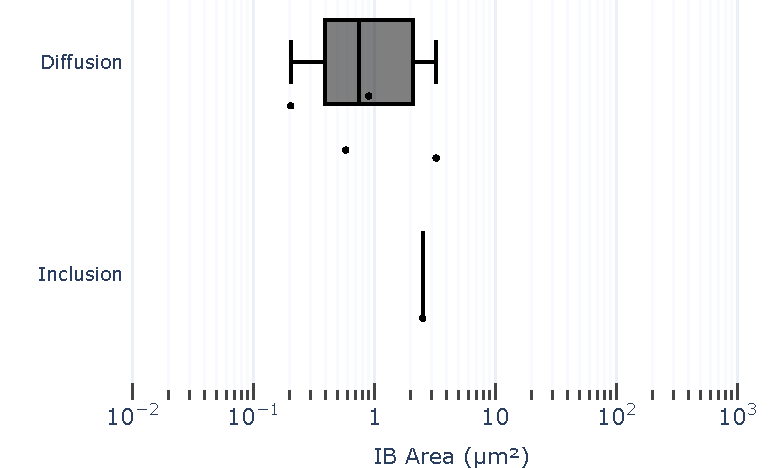
\includegraphics[width=1\linewidth]{09. Chapter 4/Figs/02. Overexpression/04. IFIT5/05. box_i5_brsv.pdf}
    \end{subfigure}
    \caption[Observed Phenotypes of Exogenous hIFIT5 in the Context of bRSV Inclusion Bodies in Vero Cell Line.]{\textbf{Observed Phenotypes of Exogenous hIFIT5 in the Context of bRSV Inclusion Bodies in Vero Cell Line.} Vero cells were infected with bovine RSV at MOI 1. 24 HPI, the cells were transfected with hIFIT5-FLAG containing plasmids using TransIT-X2 and were fixed after further 24 hours. Cells were labeled with anti-RSV N and anti-FLAG antibodies and imaged on confocal microscope. Panel (a) shows percentual proportions of observed phenotypes between bRSV inclusion bodies and exogenous hIFIT5 (5 observations), with the red dotted line denoting the 5\% threshold, marking phenotypes considered relevant above this limit. Panel (b) shows the IB area in \(\mu \mbox{m}^2\) per observed relevant phenotype.}
    \label{fig:Observed Phenotypes of Exogenous hIFIT5 in the Context of bRSV Inclusion Bodies in VERO Cell Line}
\end{figure}

\begin{figure}
    \centering
    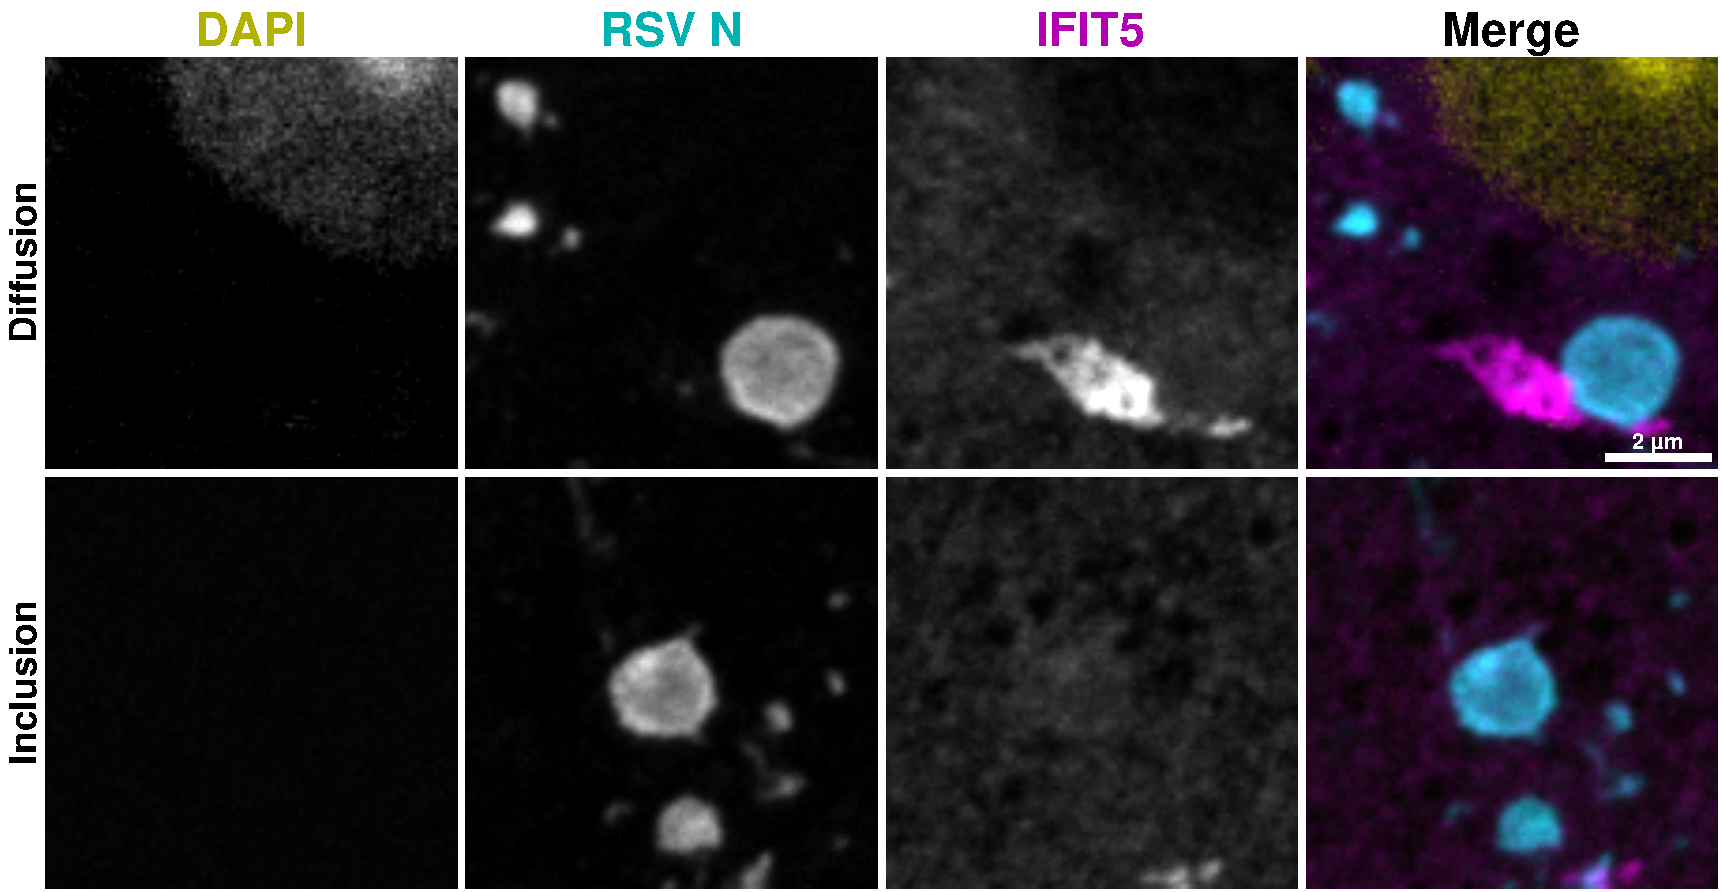
\includegraphics[width=1\linewidth]{09. Chapter 4/Figs/02. Overexpression/04. IFIT5/06. i5-brsv.pdf}
    \caption[Representative Images of Observed Phenotypes of Exogenous hIFIT5 in the Context of bRSV Inclusion Bodies in Vero Cell Line.]{\textbf{Representative Images of Observed Phenotypes of Exogenous hIFIT5 in the Context of bRSV Inclusion Bodies in Vero Cell Line.} Vero cells were infected with bovine RSV at MOI 1. 24 HPI, the cells were transfected with hIFIT5-FLAG containing plasmids using TransIT-X2 and were fixed after further 24 hours. Cellular nuclei were stained with DAPI (yellow), and cells were double-labeled with anti-RSV N (cyan) and anti-FLAG (magenta) antibodies. This figure showcases representative examples of relevant phenotypes in the interaction between exogenous hIFIT5 and bRSV inclusion bodies. These phenotypes are presented in descending order based on their percentage proportions. The scale bar indicates 2 \(\mu \mbox{m}\).}
    \label{fig:Representative Images of Observed Phenotypes of Exogenous hIFIT5 in the Context of bRSV Inclusion Bodies in VERO Cell Line}
\end{figure}

Finally we have investigated the intraction betwenn exogenously expressed human IFT5 and bRSV IBs. We have observed only 5 IB/IFIT5 interactions. Regardless, the observed phenotypes, their frequency of occurance, along with the measured IB areas are shown in Figure \ref{fig:Observed Phenotypes of Exogenous hIFIT5 in the Context of bRSV Inclusion Bodies in VERO Cell Line}, with the representative images of these phenotypes shown in Figure \ref{fig:Representative Images of Observed Phenotypes of Exogenous hIFIT5 in the Context of bRSV Inclusion Bodies in VERO Cell Line}. The most commonly occuring phenotypic interaction was diffusioin, which occured in 80\% of observations. IBs associated with this phenotype ranged from 0.2 \(\mu \mbox{m}^2\) to supra 3 \(\mu \mbox{m}^2\) in size, with the median measured area of 0.7 \(\mu \mbox{m}^2\). Following this we have observed one IB of 2.3 \(\mu \mbox{m}^2\) in size, inside which hIFIT5 was  observed to be concentrating and forming intra-IB inclusion. These seems to be a hint of phenotype separation based on IB size, similar to what we observed previoiously with hRSV infecton (Figure \ref{fig:Observed Phenotypes of Exogenous hIFIT5 in the Context of hRSV Inclusion Bodies in VERO Cell Line}), however this is difficult to completely assess based on 5 observations. Along this linesm we have failed to observe IBs larger than 4 \(\mu \mbox{m}^2\). Based on the hRSV results we hypothetise that these IBs would shown colocalisaton associated with exclusion phenotype.

Overall we have observed overexpressed human IFIT1 to be mainly forming intra-IB inclusions, to be diffusied equaly between the cytoplasm and the IBs, and to be colocalisng wth the edge of the large IBs, while being excluded from the ionterior of these structures. This was consistent between hRSV and bRSV infection, however we detcted more larger IBs in bRSV infection and thus observed more colocalisation associated with exclusion phenotype. Overexpressed bovine IFIT3 was observed to be mainly diffused thought the hRSV and bRSV IBs, although we have also observed it to be excluded from these structures or to be associated with the IB edges, while being excluded from the IB interior. We have observed a striking difference between the sizes of IB associated with these phenotypes between hRSV and bRSV infected samples. While there was no difference between the sizes of hRSV IB with regards to their interaction phenotype association, we have observed a clear differentiation of bIFIT3-bRSV IB interaction phenotypes based on the IB sizes. We have observed the diffusion phenotype to appear predominatly in small, immature IBs, while the colocalisation associated with exclusion and exclusioon phenotype happened in progressvely larger IBs. We have observed exogenously expressed human IFIT5 to mainly present strong interaction phenotypes with regards to hRSV IBs i.e. inclusion and colocalisation associated with exclusion phenotypes. We have however also observed diffusion phenotype to occurr. With regards to the overexpressed hIFIT5 interaction with bRSV IBs, we have obtained only a limited amount of observations. These suggested that the prevelant phenotypes are diffucion with occasional inclusion. It is however possible that gathering larger dataset with regards to the quantity and range of IB sizes we would would be able to replicate the results obtained using hRSV. Lastly we have failed to observe large IBs (i.e. more than 10 \(\mu \mbox{m}^2\)) in all condtitions but exogenously expressed human IFIT1 during bRSV infection. This is unusual as one would expect the inclusion bodies to more prevelantly larger at the timepoint of 48 HPI. This could be due to the limited observations that we have gathered and repeating the experiments and increasing the sample size could show more larger IBs. On the other hand, it is possible that the high expression of these IFITs is acting antiviraly against the RSV and is thus preventing the formation of larger IBs.